\documentclass{article}
\usepackage{graphicx}
\usepackage{multicol}
\usepackage{amsmath}
\usepackage{wasysym}
\usepackage{amssymb}
\usepackage{mathtools}
\usepackage[utf8]{inputenc}
\usepackage{setspace}
\usepackage{tabularx}
\usepackage{changepage}
\doublespacing
\usepackage[dvipsnames]{xcolor}
\newcommand{\ihat}{\mathbf {\hat \imath}}
\newcommand{\jhat}{\mathbf {\hat \jmath}}
\newcommand{\nhat}{\mathbf {\hat n}}
\DeclareMathOperator{\dis}{d}
\newcommand{\vect}[1]{\mathbf{#1}}
\newcommand{\beginsp}[1]{\begin{adjustwidth}{2.5cm}{2.5cm}#1\end{adjustwidth}}
\newcommand{\definition}[2]{\textbf{Definition. #1.}\begin{adjustwidth}{1cm}{1cm}#2\end{adjustwidth}}
\newcommand{\theorem}[2]{\textbf{Theorem. #1.}\begin{adjustwidth}{1cm}{1cm}#2\end{adjustwidth}}
\newcommand{\lemma}[2]{\textbf{Lemma. #1.}\begin{adjustwidth}{1cm}{1cm}#2\end{adjustwidth}}
\newcommand{\corollary}[2]{\textbf{Corollary. #1.}\begin{adjustwidth}{1cm}{1cm}#2\end{adjustwidth}}
\rmfamily
\setlength{\parindent}{0pt}
\usepackage{geometry}
\geometry{
	paper=a4paper,
	top=2.54cm,
	bottom=2.54cm,
	left=2.54cm, 
	right=2.54cm, 
	headheight=14pt, 
	footskip=1.2cm,
	headsep=1.2cm, 
}

\begin{document}
\begin{titlepage}
    \centering
    \vspace*{\fill}

    \vspace*{0.5cm}

    \huge\bfseries
    Higher Linear Algebra\\Definitions and Theorems

    \vspace*{2cm}

    \large Dylan Wang (z5422214)

    \vspace*{2cm}

    \large May 2023, Term 2

    \vspace*{\fill}
\end{titlepage}
\newpage
\definition{Groups}{A group $G$ is a non-empty set with a binary operation defined on it. That is \begin{enumerate} \item Closure: for all $a$, $b \in G$ a composition $a * b$ is defined and in $G$.\item Associativity: for all $a,b \in G$, $(a*b)*c=a*(b*c)$. \item Identity: There is an element $e \in G$ such that $a * e e * a = a$. \item Inverse: for each $a \in G$ there exists an $a' \in G$ such that $a * a' = a' * a = e*.$ \end{enumerate}If $G$ is a finite set then the order of $G$ is $|G|$, the number of elements in $G$. Technically, a group is the pair $(G, *)$; said as ``the group $G$ under the operation $*$''.\\[1\baselineskip]\textsuperscript{*}it captures the idea of a collection of objects, and came from symmetry; think about actions on a structure, and composing these actions.}~\\
\definition{Abelian Group}{A group $G$ is abelian if the operation satisfies the commutative law \[a * b = b * a \qquad \text{for all} \qquad a,b \in G.\]}
\textbf{Notes on Groups}\begin{itemize}
  \item A composition is a function $*: G \times G \rightarrow G$.
  \item The operation $*$ is not restricted to but it s commonly addition (for abelian groups), mulitiplication (often written as juxtaposition) or composition of functions.
  \item We use power notation for repeated compositions: $a * a * a * \ldots * a = a^n$ and $a^{-n} = (a^{-1})^n$.
\end{itemize}
\textbf{Examples}\begin{itemize}
  \item $(\mathbb{Z}, +)$ is an abelian group;
  \item $(\mathbb{Z}, -)$ is not a group because the inverse of $2$ (or any $n \in \mathbb{Z}, n \neq \pm 1$) is not an integer.
  \item For any integer $m$, the set $\mathbb{Z}_m = \{0, 1, 2, \ldots, m-1\}$ of remainders modul $m$ is a group under addition modulo $m$.
  \item If $p$ is prime, $\mathbb{Z}^*_p = \mathbb{Z}_p \ \{0\}$ is a group under multiplication modulo $p$. This only works for primes because non-primes will lead to a zero result (e.g. $p = 6$, $2 * 3 = 6 \mod 6 = 0$.)
  \item For any set $S$, the set $F$ of bijective functions $f : S \rightarrow S$ is a group under composition, but is not in general abelian.
\end{itemize}
\lemma{Properties of a Group}{Let $(G, *)$ be a group.\begin{itemize}\item There is only one identity element in $G$.\item Each element of $G$ has only one inverse. \item For each $a \in G$, $(a^{-1})^{-1} = a$. \item For every $a,b \in G$, $(a * b)^{-1} = b^{-1} * a^{-1}$. \item Let $a,b,c \in G$. Then if $a * b = a * c$, $b = c$.Similarly, if $b * a = c * a$ then $b = c$.\end{itemize}}
\textbf{Example.}
Let $m$ be a positive integer and consider the set \[C_m = \{e, a, a^2, a^3, \ldots, a^{m-1}\},\]where $a$ is some (undefined) symbol.\\Define an operation on $C_m$ by specifying that $a^0 = e$ (soon; $a^m = e$) and \[a^k * a^l = \begin{cases}
  a^{k+l} & \text{if } k + l < m\\
  a^{k+l-n} & \text{otherwise}
\end{cases}.\]This is an abelian group known as a cyclic group of order $m$ and we often write $C_m$ as $<a: a^m = e>$ and say it is generated by $a$. \\[1\baselineskip]
\definition{Permutation Groups}{Let $\Omega_n = \{1, 2, \ldots,n\}$. As an ordered set, $\Omega_n$ has $n!$ arrangements or permutations. If we think of these as functions, then each permutation is a bijection on $\Omega_n$ (mapping indices).\\[1\baselineskip]Then the set $\mathcal{S}_n$ of all permutations of $n$ objects forms a group under composition of order $n!$. The proof follows from the bijective function on a set example.}~\\
\definition{Small Finite Groups}{A Cayley table shows the compositions associated with a group, usually for small, finite groups.\\[1\baselineskip]Each row must be a permutation of the elements of the group, because:
\begin{itemize}
  \item If we had a repitition in a row (or column), so that $x*a = x*b$, then the cancellation rule will give $a = b$.
  \item If $a^2 = a$ then composing with $a^{-1}$ gives $a = e$, so the identity is the only element that can be fixed.
\end{itemize}}
\textbf{Example.}
\begin{center}
  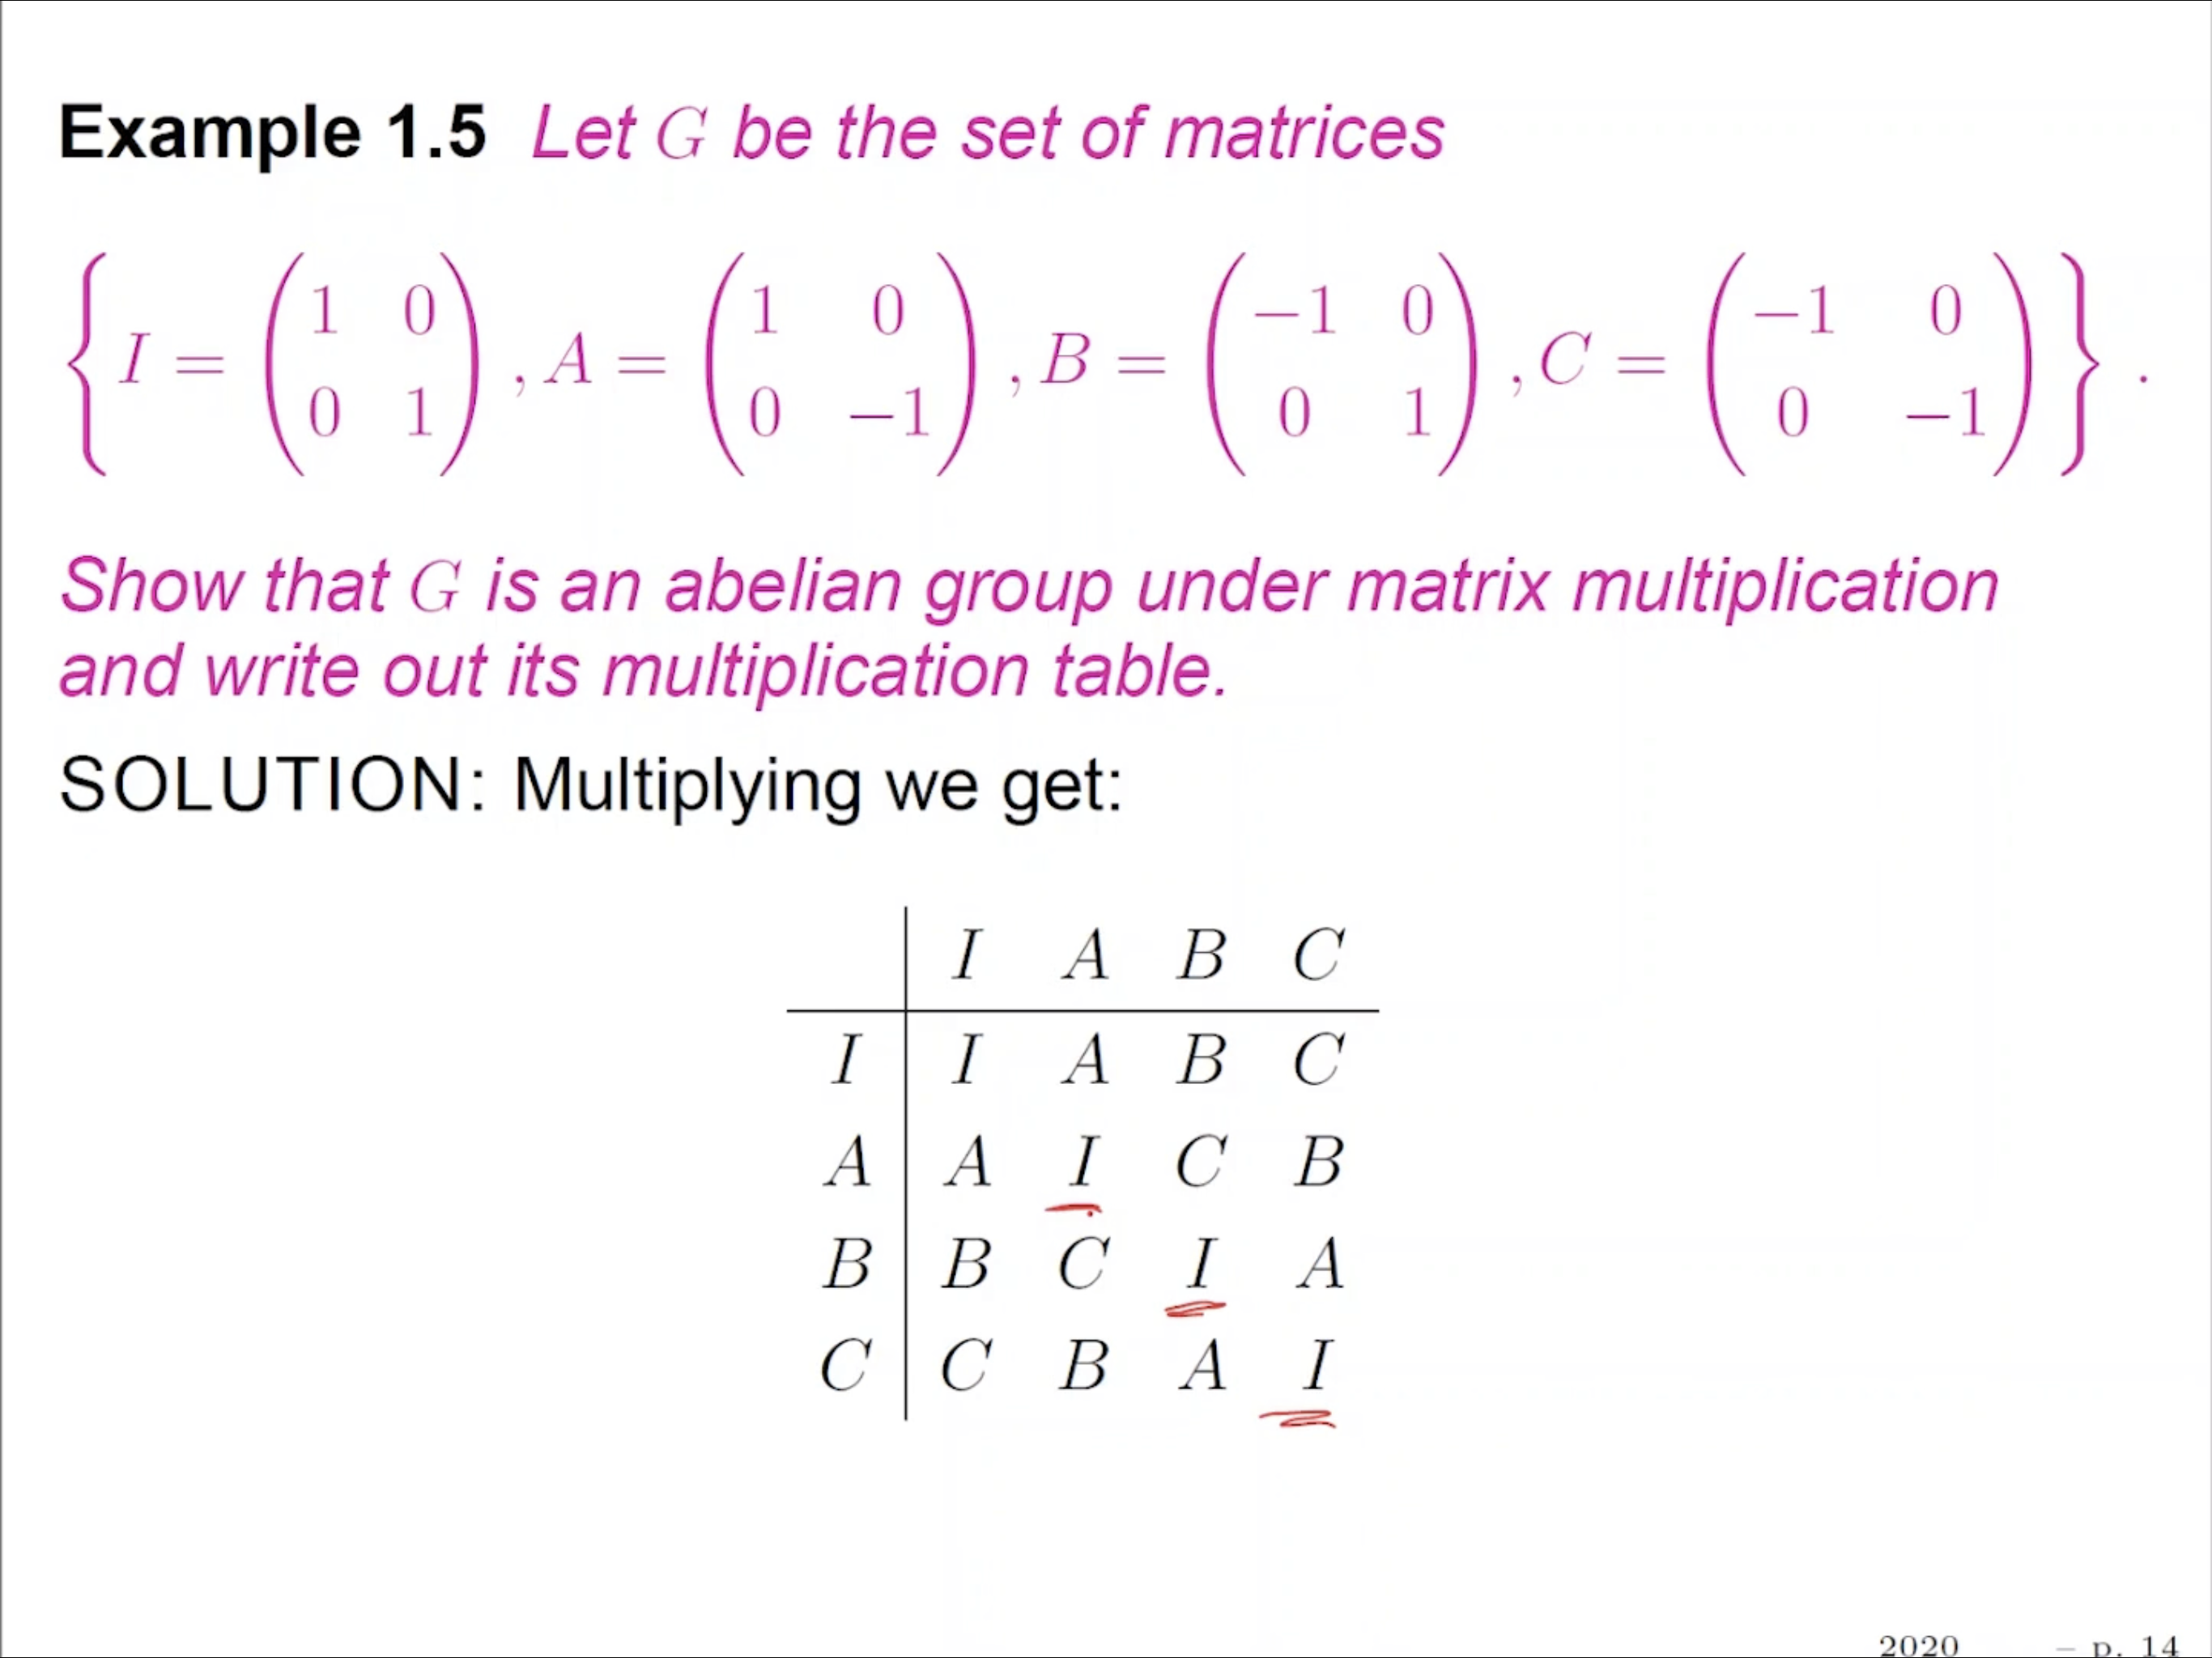
\includegraphics[scale=0.25]{assets/group_example.png}
\end{center}
\definition{Fields}{A field $(\mathbb{F}, +, \times)$ is a set $\mathbb{F}$ with two binary operations on it, addition $(+)$ and multiplication $(\times)$, where\begin{enumerate}\item $(\mathbb{F}, +)$ is an abelian gruop;\item $\mathbb{F}^* = \mathbb{F} \ \{0\}$ is an abelian group under multiplication, with $0$ being the additive identity;\item The distributive laws $a \times (b + c) = a \times b + a \times c$ and $(a + b) \times c = a \times c + b \times c$ hold.\end{enumerate}Note this satisfies the $12=5 + 5 + 2$ number laws.\\[1\baselineskip]\textsuperscript{*}it is called a `field' to resemble fields in physics; that is, a premise upon which there is rich structure and interplay.}~\\
\lemma{Interplay Between $+$ and $\times$}{Let $\mathbb{F}$ be a field and $a,b,c \in \mathbb{F}$. Then\begin{itemize}\item $a0 = 0$ (additive identity); \item $a(-b) = -(ab)$ (associativity); \item a(b-c) = ab - ac (distributive law); \item if $ab = 0$ then either $a = 0$ or $b = 0$ (proof: suppose $ab = 0$ and $a \neq 0$, then multiply both sides by $a^{-1}$ to give $0 = a^{-1}0 = a^{-1}(ab) = (a^{-1}a)b = 1b = b)$.\end{itemize}}~\\
\definition{Subgroups}{Let $(G,*)$ be a group and $H$ a non-empty subset of $G$.\\Then $H$ is a subgroup of $G$ if $H$ is a group under the restriction of $*$ to $H$.\\We write this as $H \leq G$ and say $H$ inherits the group structure from $G$.\\[1\baselineskip]\textsuperscript{*}the idea is that $H$ is just a smaller bunch of objects within $G$, the whole collection, and also has its structure and properties.}~\\
\lemma{The Subgroup Lemma}{Let $(G, *)$ be a group and $H$ and non-empty subset of $G$.\\Then $H$ is a subgroup of $G$ if and only if \begin{itemize}
  \item for all $a,b \in H$, $a * b \in H$;
  \item for all $a \in H$, $a^{-1} \in H$;
\end{itemize}These are all proved from closure and inverse of the group; associativity is inherited from $G$ and an identity exists via the inverse.\\[1\baselineskip]Note that any subgroup of an abelian group is also an abelian group.}~\\
\textbf{Examples}\begin{enumerate}
  \item Every non-trivial group $G$ has at least two subgroups: $\{e\}$ and $G$.
  \item For any integer $m$ let $m\mathbb{Z}$ be the set of all multiples of $m$. Then $(m\mathbb{Z}, +)$ is a subgroup of $(\mathbb{Z}, +)$. The converse is also true; any subgroup of $(\mathbb{Z}, +)$ is $(m\mathbb{Z}, +)$ for some $m$.
  \item Consider $C_m = <a : a^m = e>$ the cyclic group of order $m$.\\Picking any integer $k$ with $1 < k < m$ we could generate a subgroup $H_k = <a^k>$ of $C_m$ by looking at all powers of $a_k$. Clearly, the order of $H_k$ cannot be larger than $m$; it is strictly less than $m$ if and only if $k$ and $m$ have a common divisor $d > 1$.
  \item Let $n \geq 1$ be any integer. The set of invertible $n \times n$ matrices over a field $\mathbb{F}$ s a group under matrix multiplication. It is non-abelian if $n > 1$. It is called the general linear group GL$(n, \mathbb{F})$.\\They have important subgroups, such as the special linear groups SL$(n,\mathbb{R})$ and SL$(n, \mathbb{C})$ of matrices with determinant $1$, and the group of orthogonal matrices $O(n) \leq$ GL$(n, \mathbb{R})$.
\end{enumerate}\newpage
\definition{Subfields}{If $(\mathbb{F}, +, \times)$ is a field and $\mathbb{E} \subseteq \mathbb{F}$ is also a field under the same operations, then $(\mathbb{E}, +, \times)$ is a subfield of $(\mathbb{F}, +, \times)$, usually written $\mathbb{E} \leq \mathbb{F}$.}~\\
\lemma{The Subfield Lemma}{Let $\mathbb{E} \neq \{0\}$ be a non-empty subset of field $\mathbb{F}$.\\Then $\mathbb{E}$ is a subfield of $\mathbb{F}$ if and only if for all $a,b \in \mathbb{E}$ \[a + b \in \mathbb{E}, \quad -b \in \mathbb{E}, \quad a \times b \in \mathbb{E}, \quad b^{-1} \in \mathbb{E} \; \text{if} \; b \neq 0.\]Proof: The distributive laws are inherited from $\mathbb{F}$, and the rest of the proof comes from applying the subgroup lemma to $(\mathbb{E}, +)$ and $(\mathbb{E}, \times)$.}~\\
\definition{Morphisms}{Let $(G, *)$ and $(H, \circ)$ be two groups. A (group) homomorphism from $G$ to $H$ is a map $\phi : G \rightarrow H$ that respects the two operations, that is where \[\phi(a * b) = \phi(a) \circ \phi(b) \quad \text{for all} \; a,b \in G.\]A bijective homomorphism $\phi: G \rightarrow H$ is called an isomorphism; the groups are then said to be isomorphic, and are considered the same group. Isomorphism is an equivalence relation.\\[1\baselineskip]\textsuperscript{*}the word `homomorphism' comes from the Ancient Greek language: homos meaning `same' and morphe meaning `form' or `shape'.\\[1\baselineskip]\textsuperscript{**}Homomorphic maps preserve the structure of the domain group while respecting that of the codomain. The idea is if $a * b$, then under the map $\phi$, we hope that (mapped) $a$ behaves the same with (mapped) $b$ in the codomain. If so, they are homomorphic.}~\\
\textbf{Example}. Let $m \geq$ 2 be any integer. Define $\phi: (\mathbb{Z},+) \rightarrow (m\mathbb{Z},+)$ by $\phi(a) = ma$. Show that $\phi$ is an isomorphism of groups.\\
\textbf{Solution.} Firstly \[\phi(a+b)=m(a+b)=ma+mb=\phi(a)+\phi(b).\]The easiest way to show $\phi$ is a bijection is to find the inverse. But if $g \in m\mathbb{Z}$ then $g=ma$ for some $a \in \mathbb{Z}$ and clearly $\phi(a) = g$, so $\phi^{-1}(g) = a$. Thus $\phi$ is an isomorphism.\\[1\baselineskip]
\lemma{Homomorphism Lemma}{Let $(G, *)$ and $(H, \circ)$ be two groups and $\phi$ a homomorphism between them. Then \begin{itemize}\item $\phi$ maps the identity of $G$ to the identity of $H$.\item $\phi$ maps inverses to inverses, i.e. $\phi(a^{-1})=(phi(a))^{-1}$ for all $a \in G$.\item if $\phi$ is an isomorphism frmo $G$ to $H$ then $\phi^{-1}$ is an isomorphism from $H$ to $G$.\end{itemize}}~\\
\definition{Kernel and Image}{Let $\phi : G \rightarrow H$ be a group homomorphism, with $e'$ the identity of $H$.\\The kernel of $\phi$ is the set \[\text{ker}(\phi) = \{g \in G: \phi(g) = e' \}.\]It is the information lost in the map.\\The image of $\phi$ is the set \[\text{im}(\phi) = \{h \in H : h = \phi(g)\}, \; \text{for some} \; g \in G\].It is the approximation given by the map.}~\\
\lemma{Kernel and Image Lemma}{For $\phi : G \rightarrow H$ a group homomorphism, $\text{ker}(\phi) \leq G$ and $\text{im}(\phi) \leq H$.}~\\
\lemma{Isomorphism Lemma}{A homomorphism $\phi$ is one-to-one if and only if $\text{ker}(\phi) = \{e\}$, with $e$ the identity of $G$. If $\phi$ is one-to-one then $text{im}(\phi)$ is isomorphic to $G$.}~\\
\definition{Linear Representation of $G$ on $\mathbb{F}^n$}{If there exists a homomorphism $\phi : G \rightarrow$ GL$(n, \mathbb{F})$ for some $n$ and some field $\mathbb{F}$, then the group im$(\phi)$ is called a linear representation of $G$ on $\mathbb{F}^n$.\\If $\phi$ is one-to-one (so every element maps to a distinct matrix), we call the representation faithful.}~\\
\definition{Permutation Representation}{From above, in the case where $G$ is finite and $H$ is $\mathcal{S}_n$ for some $n$, then we get a permutation representation of the group $G$ as a subgroup of $S_n$.}\newpage
\definition{Vector Space}{Let $\mathbb{F}$ be a field. A vector space over the field $\mathbb{F}$ consists of an abelian group $(V, +)$ and a function from $\mathbb{F} \times V$ to $V$ called scalar multiplication and written $\alpha \vect{v}$ where \begin{enumerate} \item $\alpha(\beta \vect{v}) = (\alpha \beta)\vect{v}$ for all $\alpha, \beta \in \mathbb{F}$ and $\vect{v} \in V$. \item $1\vect{v} = \vect{v}$ for all $\vect{v} \in V$. \item $\alpha (\vect{u} + \vect{v}) = \alpha \vect{u} + \alpha \vect{v}$ for all $\alpha \in \mathbb{F}$ and $\vect{u}, \vect{v} \in V$. \item $(\alpha + \beta) \vect{u} = \alpha \vect{u} + \beta \vect{u}$ for all $\alpha, \beta \in \mathbb{F}$ and $\vect{u} \in V$.\end{enumerate}There are ten axioms here; 5 from the abelian group, closure of scalar multiplication, and four explicit ones. The $+$ in $(V, +)$ may be distinguished as vector addition.\\[1\baselineskip]\textsuperscript{*}think of a space as a set with some added structure; i.e. an abelian group (vector addition) and a scalar multiplication function. This should be thought of quite loosely/abstractly.}~\\
\lemma{2.1}{Let $V$ be a vector space over field $\mathbb{F}$. For all $\vect{v}, \vect{w} \in V$ and $\lambda \in \mathbb{F}$ then \begin{itemize}
  \item $0\vect{v} = \vect{0}$ and $\lambda \vect{0} = \vect{0}$.
  \item $(-1)\vect{v} = -\vect{v}$.
  \item $\lambda \vect{v} = \vect{0}$ implies either $\lambda = 0$ or $\vect{v} = \vect{0}$.
  \item If $\lambda \vect{v} = \lambda \vect{w}$ and $\lambda \neq 0$ then $\vect{v} = \vect{w}$.
\end{itemize}}~\\
\textbf{Standard Vector Space Examples.}
\begin{enumerate}
  \item $n$-tuples.\begin{center}
    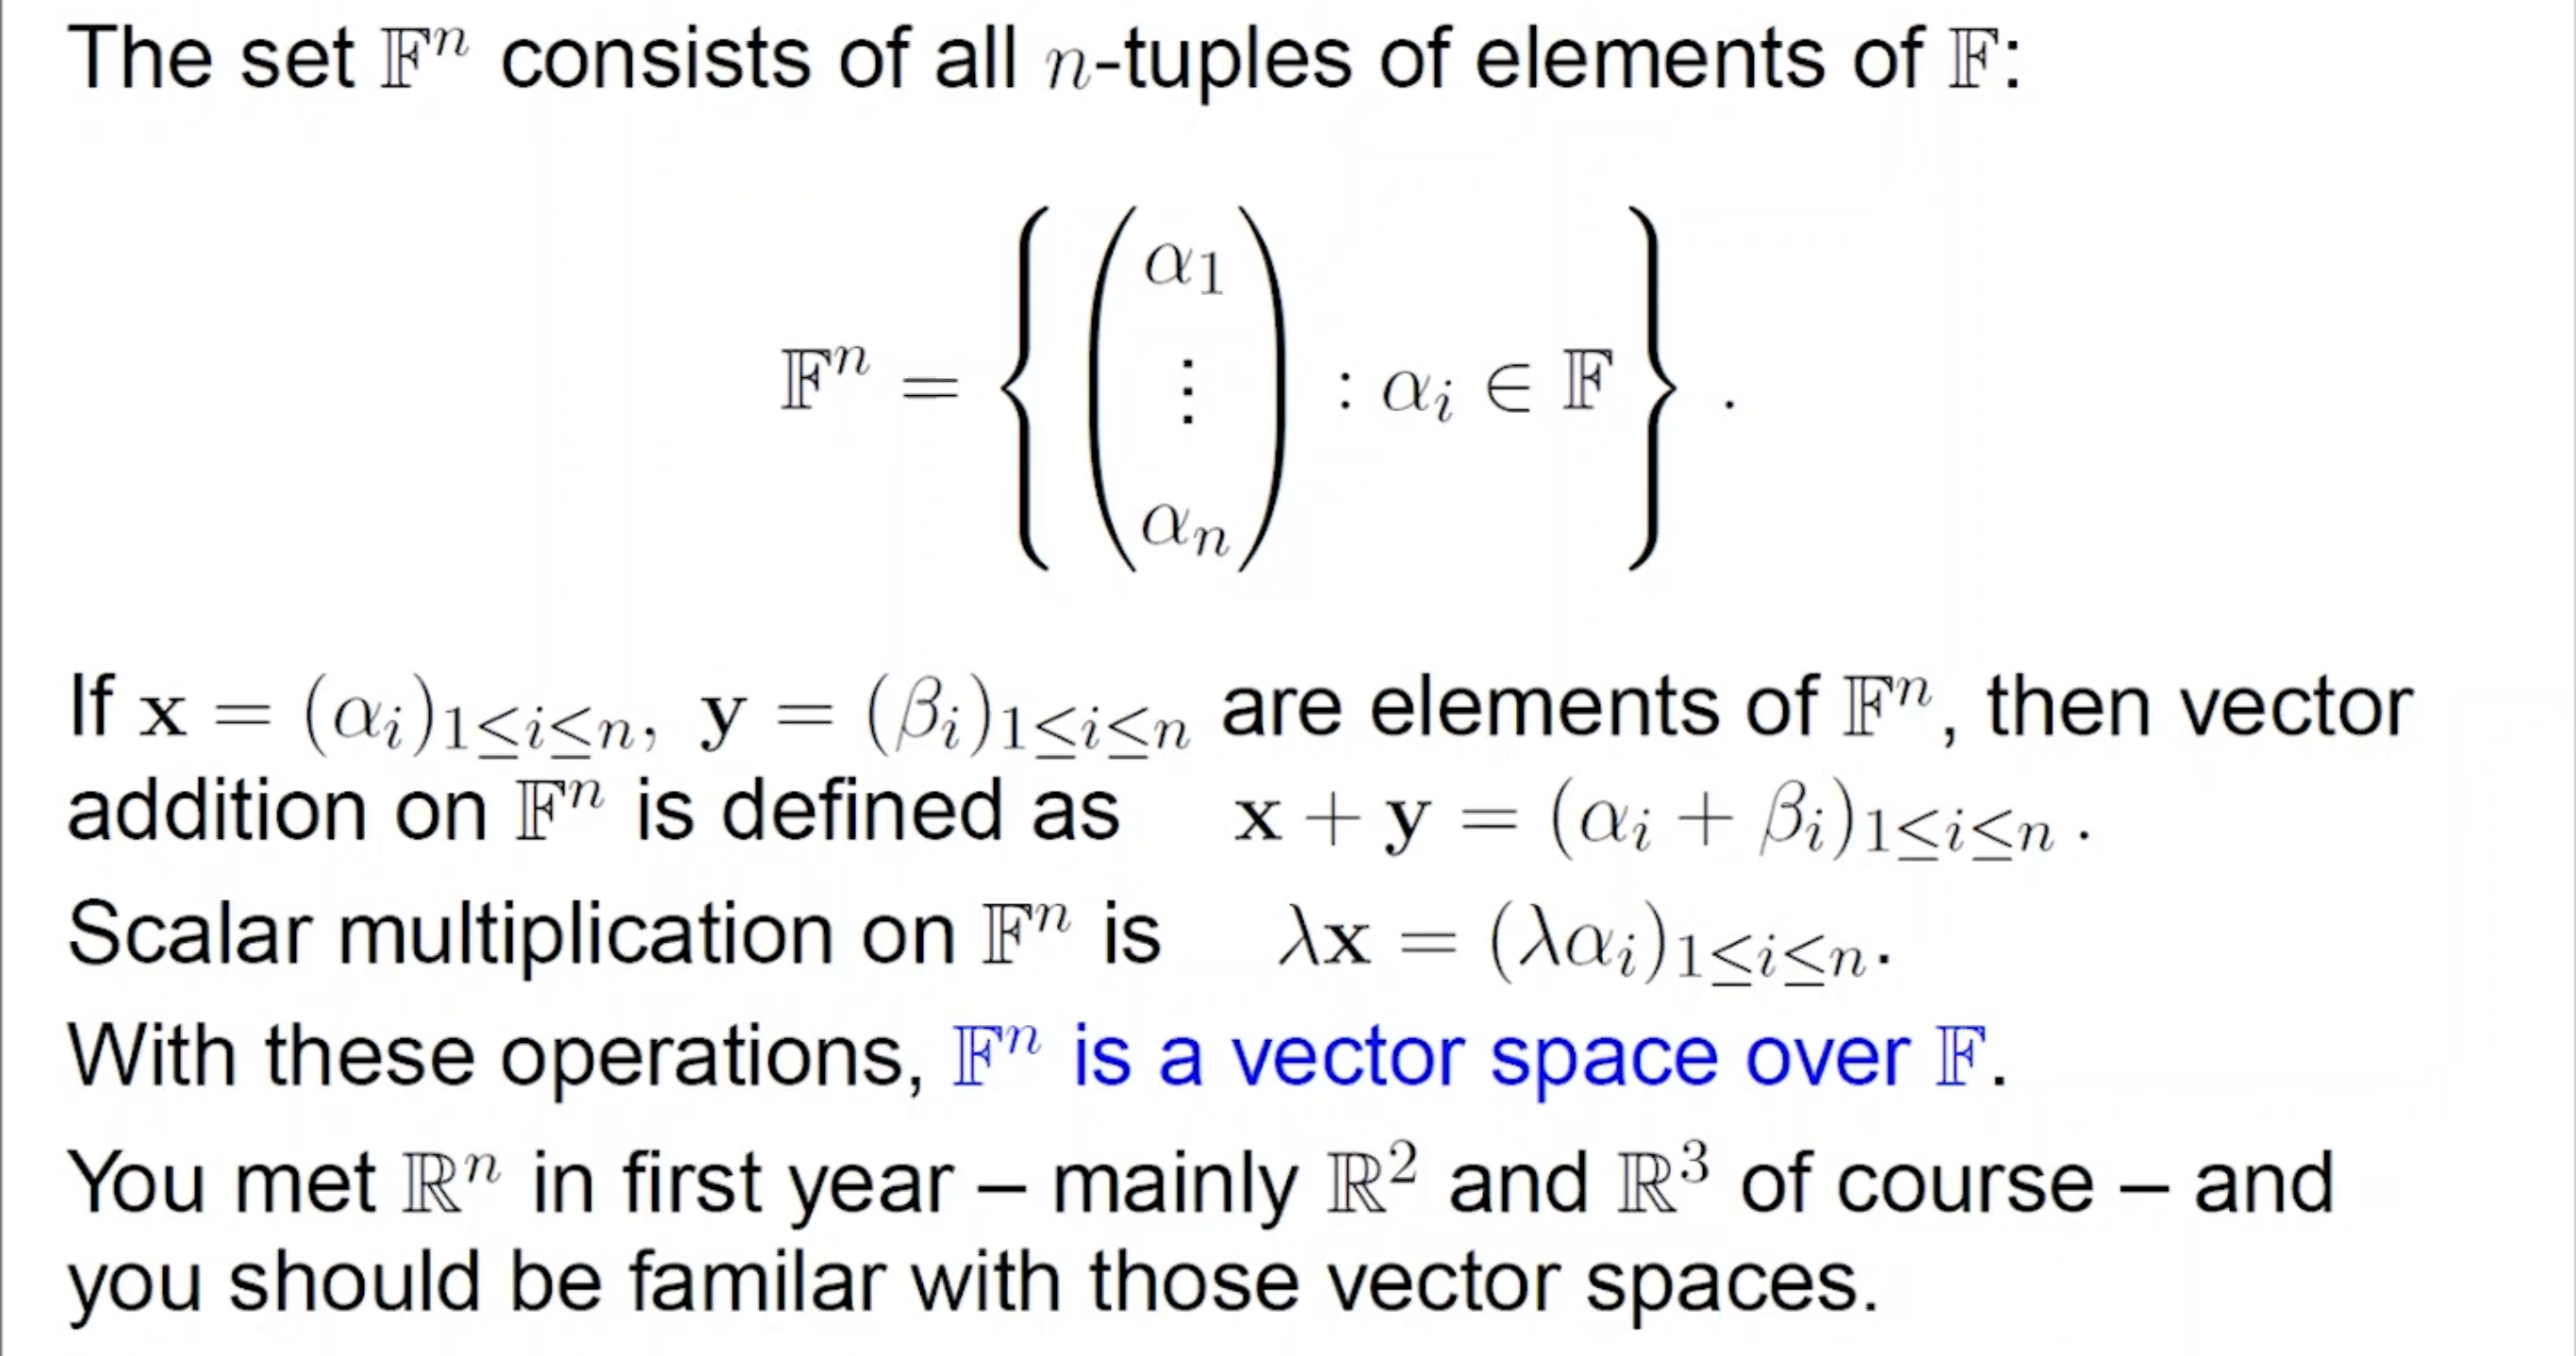
\includegraphics[scale=0.3]{assets/vector_space_eg.png}\newpage
  \end{center}
  \item Geometric Vectors.\begin{center}
    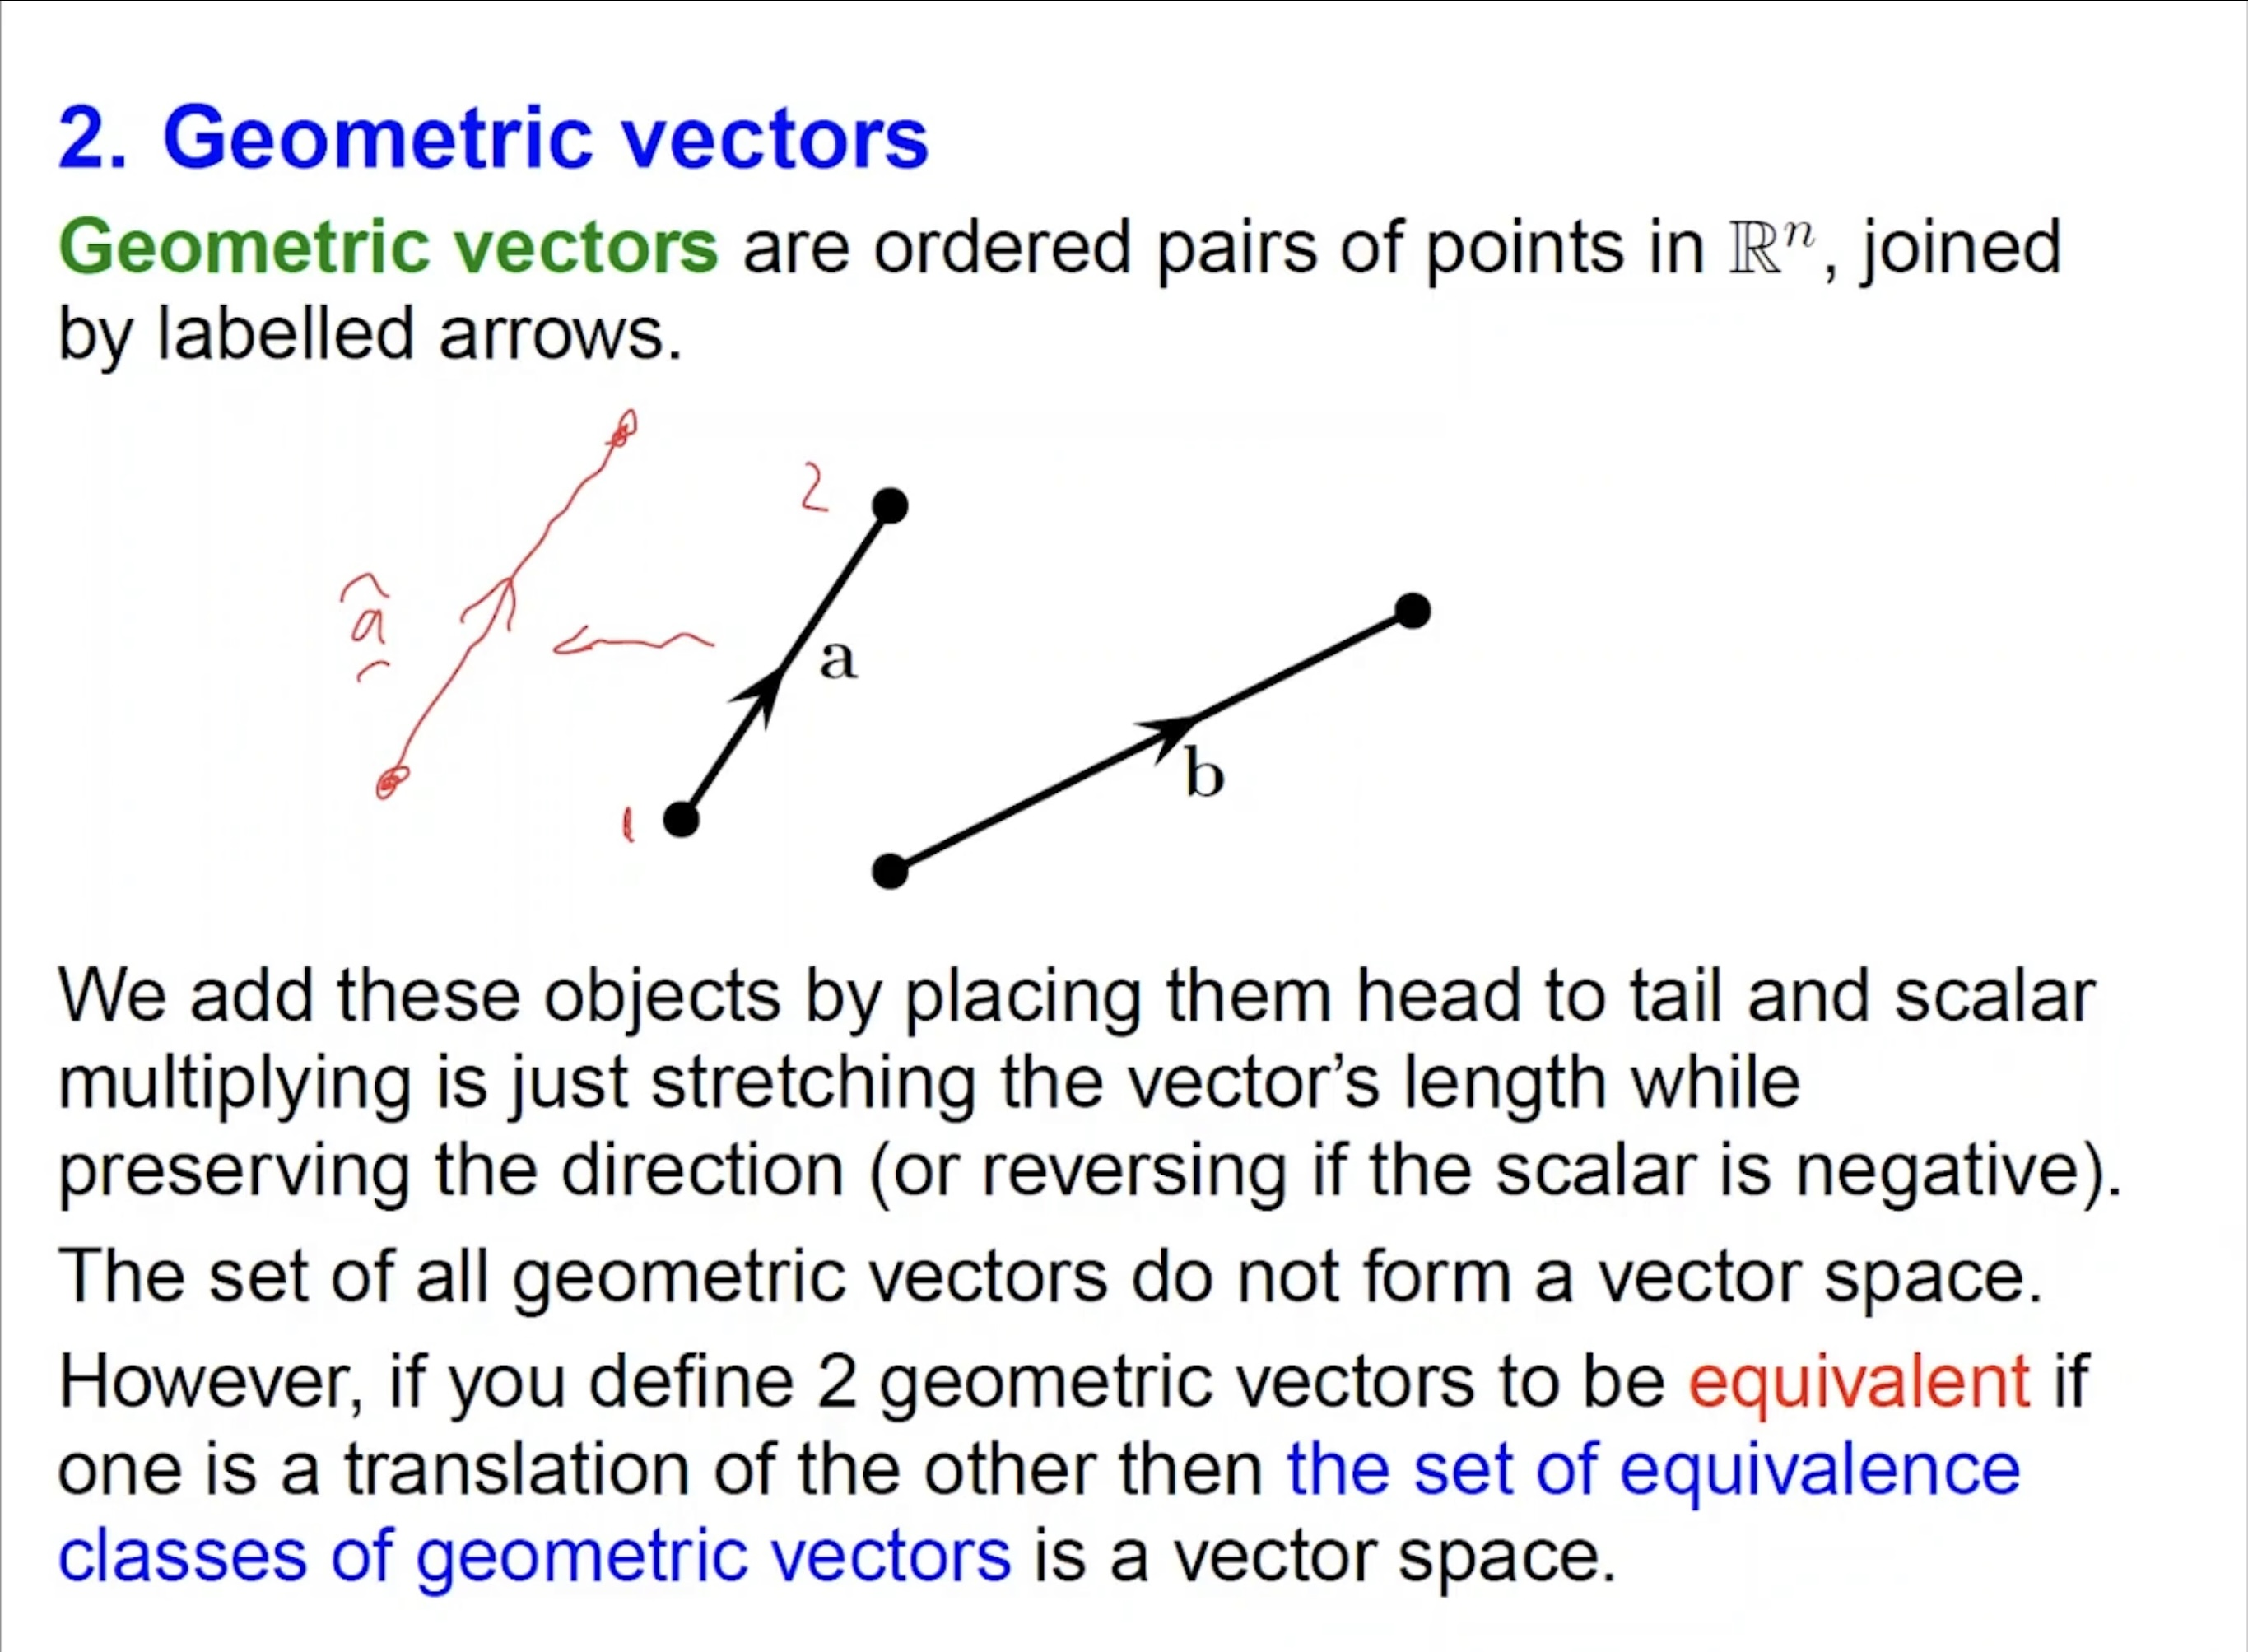
\includegraphics[scale=0.10]{assets/geometric_vecs.png}
  \end{center}
  \item Matrices.\\For any positive integers $p$ and $q$ the set $M_{p,q}(\mathbb{F})$ is the set of $p \times q$ matrices with elements from $\mathbb{F}$.\\Then $M_{p,q}(\mathbb{F})$ is a vector spsace over $\mathbb{F}$ with vector addition with the usual addition of matrices and scalar multiplication multiplying each element of the matrix.
  \item Polynomials.\\The set of all Polynomials with coefficients in $\mathbb{F}, \mathcal{P}(\mathbb{F}),$ is a vector space over $\mathbb{F}$ with \[(f+g)(x) = f(x) + g(x) \quad \text{for all} \quad x \ in \mathbb{F} \\ (\lambda f)(x) = \lambda f(x) \quad \text{for all} \quad \lambda, x \in \mathbb{F}.\]Similarly, $\mathcal{P}(F)$ (polynomials of degree $n$ or less) is a vector space over $\mathbb{F}$. Note this example shows `vector spaces' can appear abstract from actual vectors! We just need vector $+$ and $\times$.
  \item Function Spaces.\\Let $X$ be a non-empty set and $\mathbb{F}$ be a field. Then define \[\mathcal{F}[X] = \{f: X \rightarrow \mathbb{F} \}.\]The set $\mathcal{F}[X]$ is a vector space over $\mathbb{F}$ if we define \begin{itemize}\item the zero in $\mathcal{F}[X]$ to be the zero function: $x \rightarrow 0$ for all $x \in X$.
  \item $(f+g)(x) = f(x) + g(x)$ for all $x \ in X$.
  \item $(\lambda f)(x) = \lambda (f(x))$ for all $x \in X$.
  \end{itemize}
\end{enumerate}\newpage
\definition{Subspace}{If $V$ is a vector space over $\mathbb{F}$ and $U \subseteq V$, then $U$ is a subspace of $V$, written $U \leq V$, if it is a vector space over $\mathbb{F}$ with the same addition and scalar multiplication as in $V$.\\[1\baselineskip]Every vector space has $\{\vect{0}\}$, the trivial subspace, and itself as subspaces.}~\\
\lemma{Subspace Test Lemma}{Suppose $V$ is a vector space over the field $\mathbb{F}$ and $U$ is a non-empty subset of $V$. Then $U$ is a subspace of $V$ if and only if for all $\vect{u}, \vect{v}, \in U$ and $\alpha \in \mathbb{F}$, $\alpha \vect{u} + \vect{v} \in U$.\\[1\baselineskip]\textbf{Proof}: All of the axioms are inherited from $V$ except for closure and that the zero vector is in $U$. But setting $\alpha = 1$ proves $U$ is closed under addition. With $\alpha = -1$ and $\vect{v} = \vect{u}$ we get $\vect{0} \in U$. Hence we can set $\vect{v} = \vect{0}$ to get closure under scalar multiplication.}~\\
\textbf{Example.} In $\mathbb{R}^2$ consider the subset \[U = \{ \vect{x} = \begin{pmatrix} x_1 \\ x_2 \end{pmatrix} : x_1 + x_2 = 0 \}.\] Prove that $U$ is a subspace.\\
\textbf{Proof}: Clearly, $\vect{0} \in U$ so $U$ is not empty.\\Suppose $\vect{x} = \begin{pmatrix}x_1 \\ x_2\end{pmatrix}$ and $\vect{y} = \begin{pmatrix}y_1 \\ y_2\end{pmatrix}$ are in $U$, so $x_1 + x_2 = 0$ and $y_1 + y_2 = 0$.\\Then $\alpha\vect{x} + \vect{y} = \begin{pmatrix}\alpha x_1 + y_1 \\ \alpha x_2 + y_2\end{pmatrix}$ for $\alpha \in \mathbb{R}$ and $(\alpha x_1 + y_1) + (\alpha x_2 + y_2) = \alpha(x_1 + x_2) + (y_1 + y_2) = 0$.\\So $\alpha \vect{x} + \vect{y} \in U$ and $U \leq \mathbb{R}^2$.\\[1\baselineskip]
\definition{Linear Combination}{Let $V$ be a vector space over $\mathbb{F}$. A finite linear combination of vectors $\vect{v}_1, \vect{v}_2, \ldots, \vect{v}_n$ in $V$ is any vector which can be expressed\[\alpha_1 \vect{v}_1 + \alpha_2 \vect{v}_2 + \ldots + \alpha _n \vect{v}_n ,\]where the $\alpha_k$ are scalars.\\[1\baselineskip]\textsuperscript{*}think of a linear combination as a combination of linear, i.e. $\vect{v}^1$, vectors.}~\\
\definition{Span}{If $S$ is a subset of $V$, then the span of $S$ is \[\text{span}(S) = \{\text{all finite linear combinations of vectors in }S\}.\]We say that $S$ spans $V$, or is a spanning set for $V$, if span$(S) = V$.\\[1\baselineskip]\textsuperscript{*}i.e. given a subset of vectors, forming its span is essentially doing everything to the members of the set that can be done within the rules of a vector space.\\Clearly, $S \subseteq$ span$(S)$ and span$(S)$ is a subset of $V$.}~\\
\lemma{Lemma 2.3}{If $S$ is a non-empty subset of a vector space $V$, then span$(S)$ is a subspace of $V$.\\[1\baselineskip]\textbf{Proof}: Since $S \subseteq$ span$(S)$, span$(S)$ is non-empty.\\But if $\vect{v}$, $\vect{w} \in S$, then $\lambda \vect{v} + \vect{w}$ is a linear combination of two linear combinations of elements of $S$, and so is a linear combination of elements of $S$.\\Thus $\lambda \vect{v} + \vect{w} \in$ span$(S)$ and so span$(S) \leq V$.}~\\
\definition{Linear Independence}{A subset $S$ of a vector space $V$ is linearly independent if for all vectors $\vect{v}_1, \vect{v}_2, \ldots, \vect{v}_n$ in $S$ (with $n \geq 1$) the equation \[\alpha_1 \vect{v}_1 + \alpha_2 \vect{v_2} + \ldots + \alpha _n \vect{v}_n = \vect{0},\]with $\alpha _i \in \mathbb{F}$ implies $\alpha_i = 0$ for all $i = 1\ldots n$.\\[1\baselineskip]\textsuperscript{*}i.e. none of the vectors are linear combinations of each other so that none can cancel each other out, and for their sum to be zero, they must be each be multiplied by 0.}~\\
\lemma{Definition of Linear Dependence}{If $S = \{ \vect{v}_1, \ldots , \vect{v}_n \}$ is a linearly dependent set in $V$ then there is an $i$, $2 \leq i \leq n$ such that \[ \vect{v}_i = \sum_{j=1}^{i-1} \beta _j \vect{v}_j,\]i.e. at least one vector is a linear combination of its predecessors.\\\textbf{Proof}: Since $S$ is linearly dependent, there is a non trivial solution to $\alpha_1 \vect{v}_1 + \alpha_2 \vect{v_2} + \ldots + \alpha _n \vect{v}_n = \vect{0}$. For such a solution, let $i$ be the index o the last non-zero $\alpha_i$. Then $-\alpha_i \vect{v}_i = \sum_{j=1}^{i-1} \alpha_j \vect{v}_j$ and divide by $- \alpha_i$ for the result.}~\\
\theorem{Theorem 2.5}{In any vector space
\begin{itemize}
  \item Any subset of a linearly independent set is linearly independent.
  \item \begin{enumerate}
    \item If $\vect{v} \in$ span$(S)$, then $S \cup \{ \vect{v} \}$ is linearly dependent.
    \item If $S$ is linearly independent and $S \cup \{ \vect{v} \}$ is linearly dependent, then $\vect{v} \in $ span$(S)$.
  \end{enumerate}
  \item \begin{enumerate}
    \item If $S_1 \subseteq S_2$, then span$(S_1) \subseteq$ span$(S_2)$.
    \item If $S_1 \subseteq$ span$(S_2)$, then span$(S_1) \subseteq$ span$(S_2)$. \{Any linear combination of vectors in $S_1$ is a linear combination of vectors already in span$(S_2)$.\}
  \end{enumerate}
  \item span$(S) \cup \{ \vect{v} \} = $ span$(S)$ if and only if $\vect{v} \in $ span$(S)$.
  \item If $S$ is linearly dependent, then there is a vector $\vect{v}$ in $S$ such that span$(S) \backslash \{ \vect{v} \} = $ span$(S)$.
  \item In $\mathbb{F}^p$, if $P \in$ GL$(p, \mathbb{F})$ is an invertible matrix and $\{ \vect{v}_i \}$ is linearly independent, then the set $\{ P \vect{v}_i \}$ is also linearly independent. \{Proof by contradition\}.
\end{itemize}}~\\
\definition{Bases}{Let $S \subseteq V$. The set $S$ is a basis for $V$ over $\mathbb{F}$ if and only if $V =$ span$(S)$, and $S$ is a linearly dependent set.\\[1\baselineskip]\textsuperscript{*}think the `basic' foundation of a vector space; the minimal set of vectors from which we can form all vectors in $V$ via linear combinations.}
\begin{center}
  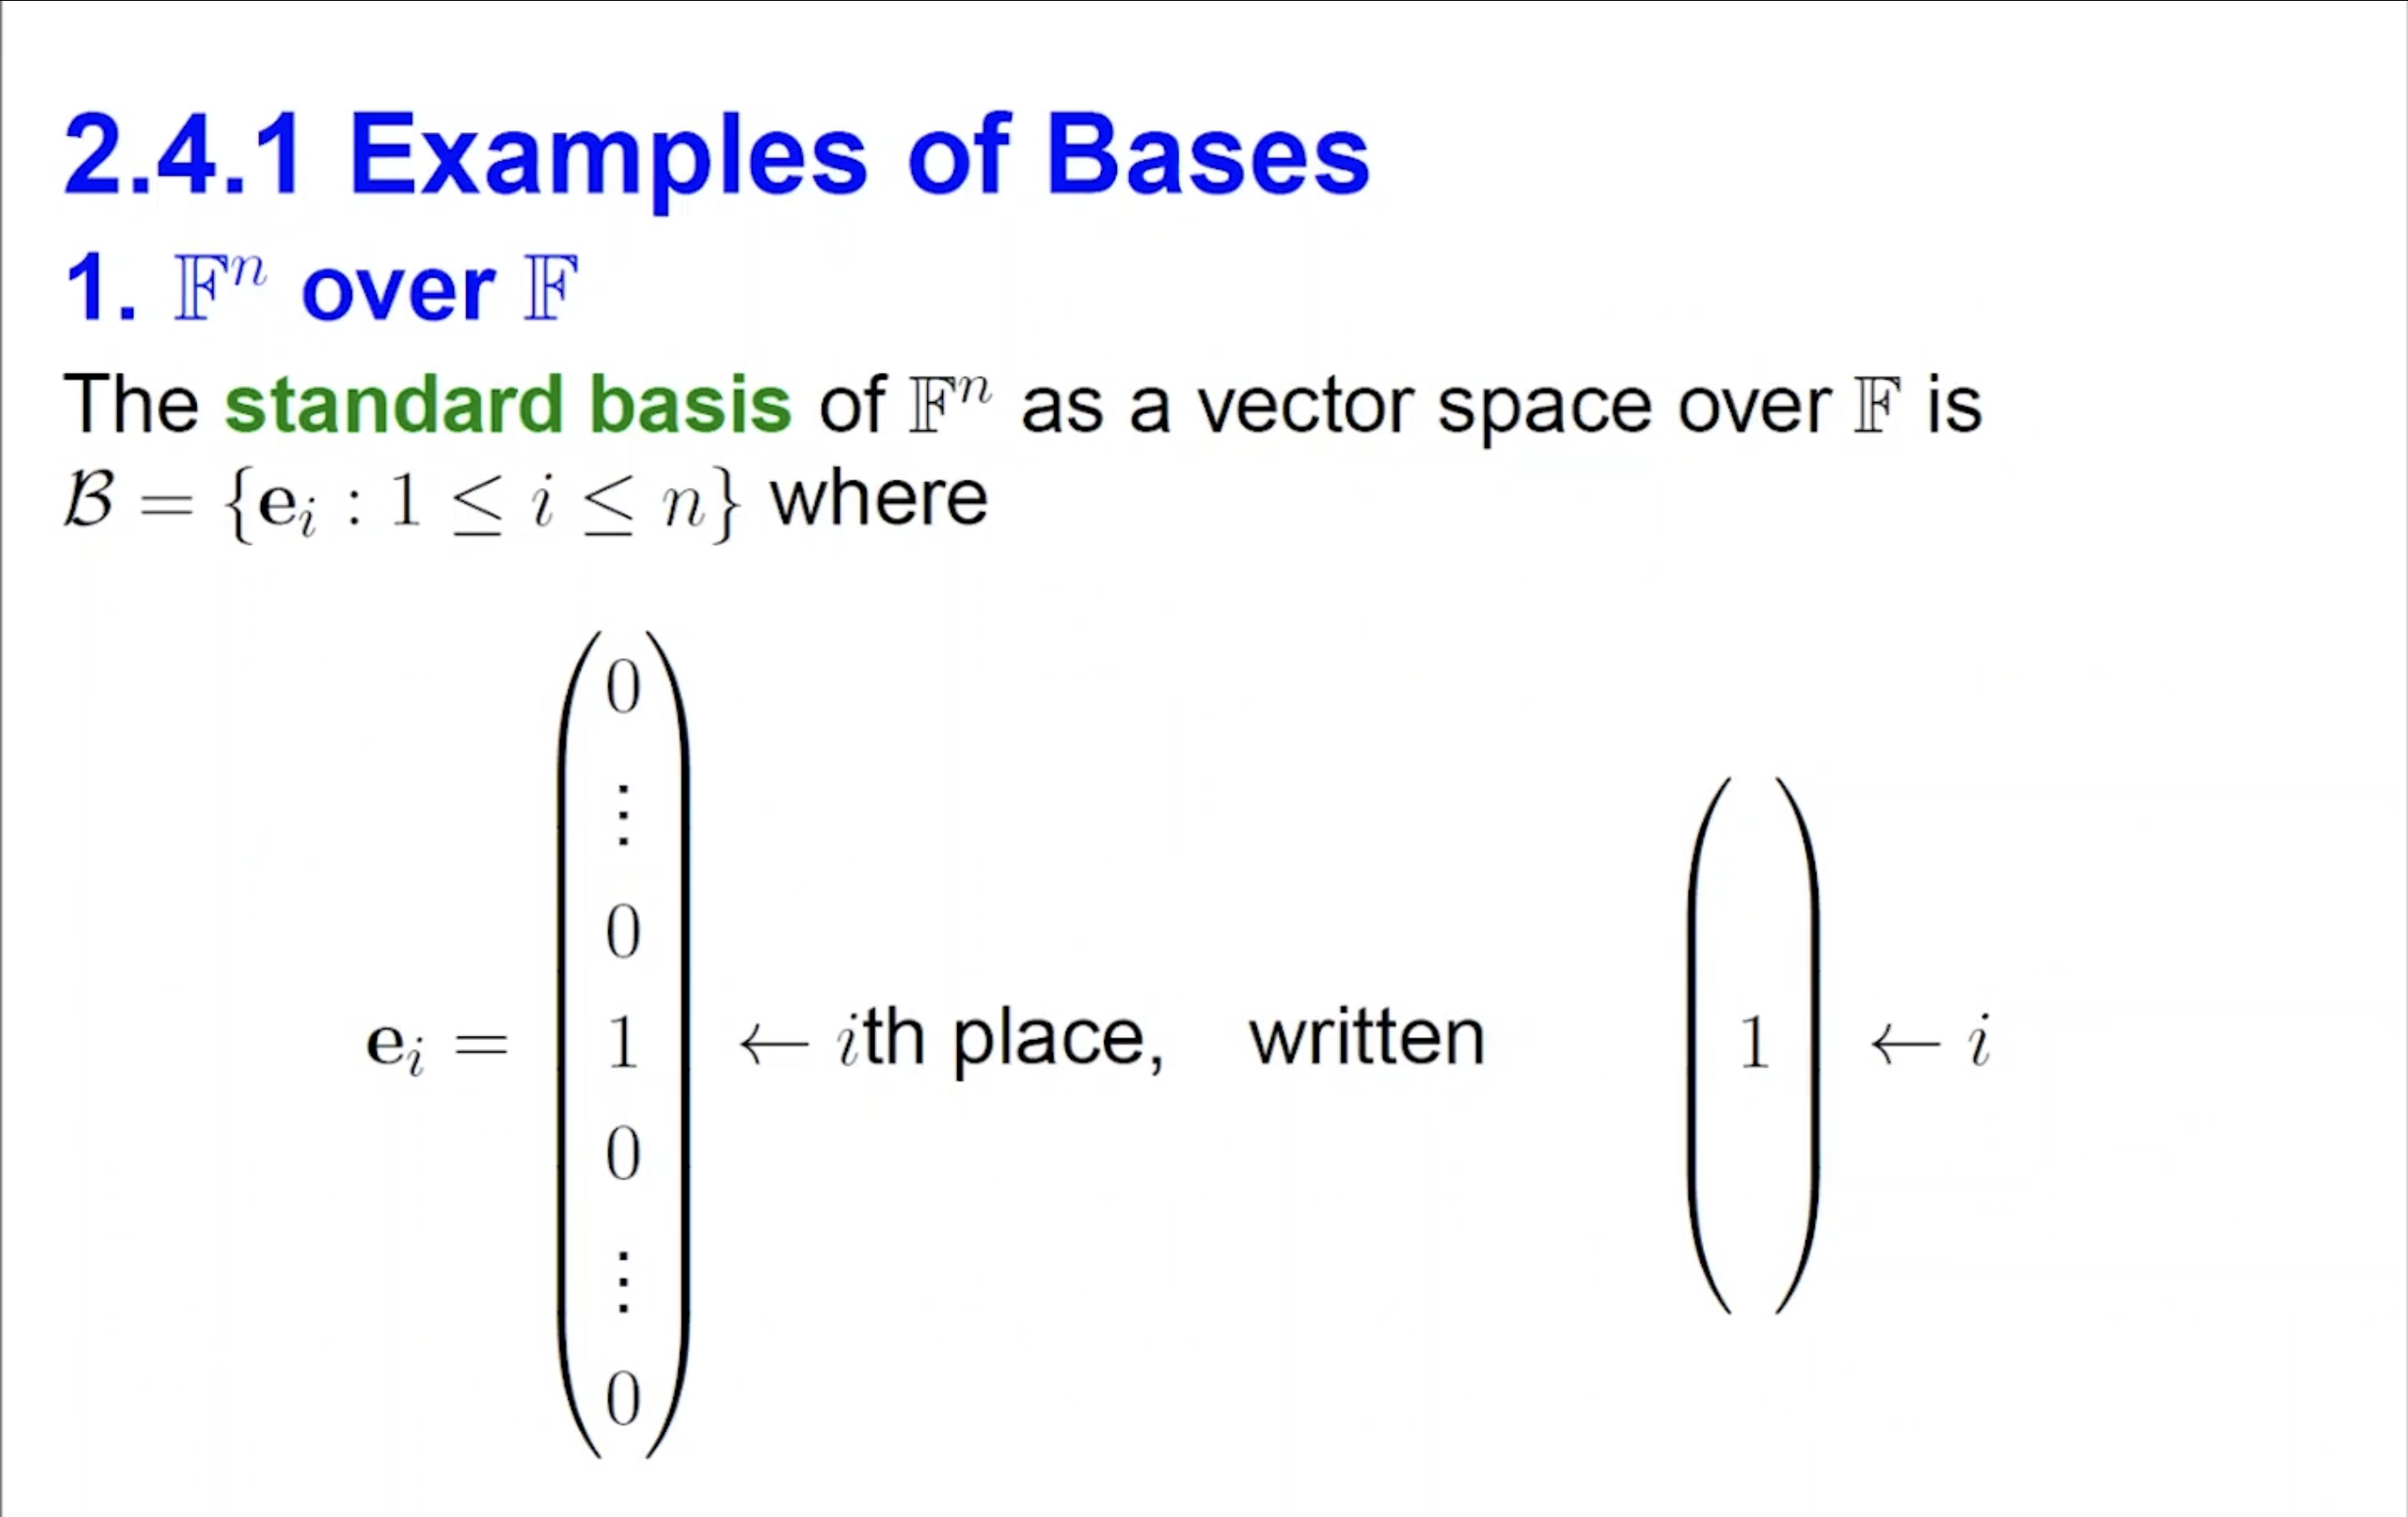
\includegraphics[scale=0.18]{assets/basis_eg.png}
\end{center}
[See Chapter 2 Video 8 of lectures for examples on matrices, polynomials, function spaces, etc.]\\[1\baselineskip]
\theorem{2.7}{Let $V$ be a vector space over $\mathbb{F}$ and $S$ a finite spanning set. Then $S$ contains a finite basis for $V$.}~\\
\lemma{The Exchange Lemma}{Suppose that $S$ is a finite spanning set for $V$ and that $T$ is a (finite) linearly independent subset of $B$ with $|T| \leq |S|$.\\Then there is a spanning set $S'$ of $V$ such that \[T \subseteq S' \quad \text{and} \quad |S'| = |S|.\]\textsuperscript{*}the intuition is we swap out one element from the finite spanning set $S$ in favour of a suitable element from a smaller linearly independent set $T$; hence the name.\\[1\baselineskip]
\textbf{Corollary. 2.9.}\\If $S$ is a finite spanning set for a vector space $V$ and $T$ is a linearly independent subset of $V$, then $T$ is finite and $|T| \leq |S|$.}~\\
\theorem{2.10}{Let $V$ be a vector space over $\mathbb{F}$ with a finite spanning set and $T$ a linearly independent subset of $V$.\\Then there is a basis $B$ of $V$ which contains $T$.\\ \textsuperscript{*}i.e. any linearly independent set can be extended to a basis (if there is a finite spanning set).}~\\ 
\theorem{2.6}{If a vector space $V$ admits a finite spanning set, it admits a finite basis and all bases contain the same number of elements.}~\\
\definition{Dimension}{The dimension of a vector space $V$ is the size of a basis if $V$ has a finite basis or infinity otherwise, denoted as dim$(V) = n$ or dim$(V) = \infty$.}~\\
\lemma{2.11}{Let $V$ be a finite dimensional vector space and suppose dim$(V) = n$. \begin{enumerate} \item The number of elements in any spanning set is at least $n$. \item The number of elements in any independent set is no more than $n$. \item If span$(S) = V$ and $|S| = n$ then $S$ is a basis. \item If $S$ is a linearly independent set and $|S| = n$ then $S$ is a basis. \end{enumerate} }~\\
\theorem{2.12}{Let $V$ be a finite dimensional vector space over $\mathbb{F}$.\\Then $\mathcal{B} = \{ \vect{v_1}, \ldots , \vect{v}_n \}$ is a basis for $V$ if and only if every $\vect{x} \in V$ can be written uniquely as $\vect{x} = \sum_{i=1}^n \alpha _i \vect{v}_i, \; \alpha _i \in \mathbb{F}$.}~\\
\definition{Coordinates}{Suppose $V$ is a vector space of dimension $n$ over $\mathbb{F}$ and suppose $\mathcal{B} = \{ \vect{v}_1, \ldots , \vect{v}_n \}$ is an ordered basis for $V$ over $\mathbb{F}$.\\If $\vect{v} \in V$ then $\vect{v} = \sum_{i=1}^n \alpha_i \vect{v}_i$ with the $\alpha_i$ unique by theorem 2.12.\\We call $\alpha = \begin{pmatrix}\alpha_1 \\ \vdots \\ \alpha_n\end{pmatrix}$ the coordinate vector of $\vect{v}$ with respect to $\mathcal{B}$, and refer to the $\alpha_i$ as the coordinates of $\vect{v}$. A useful notation is \[\vect{\alpha} = [\vect{v}]_{\mathcal{B}} \; \text{if} \; \vect{v} = \sum_{i=1}^n \alpha_i \vect{v} _i.\]\textsuperscript{*}a coordinate vector is a representation of a vector as an ordered list of numbers that describes the vector in terms of (i.e. as a linear combination of) a particular ordered basis. In some sense, every finite dimensional vector space over $\mathbb{F}$ ``is'' $\mathbb{F}^n$ for some $n = |\mathcal{B}|$.}~\\
\definition{2.8. Sum of Two Subspaces}{The sum $S + T$ of two subspaces is defined as \[S + T = \{ \vect{a} + \vect{b} : \vect{a} \in S, \; \vect{b} \in T \}.\]If $S \cap T = \{ \vect{0} \}$ then we call the sum as a direct sum and denote it as $S \oplus T$. The result in either case is a subspace.}\newpage
\lemma{2.13}{The sum of subspaces $S$ and $T$ is direct if and only if any vector $\vect{x} \in S + T$ can be written in a unique way as $\vect{x} = \vect{a} + \vect{b}, \vect{a} \in S, \vect{b} \in T$.\\[1\baselineskip]\textsuperscript{*}if a non-zero vector lies in the intersection, then it can (also) be represented as a sum of two vectors in $S$ or $T$, implying the intersection is only $\vect{0}$ for adding TWO subspaces.}~\\
\theorem{2.14}{Suppose $S$ and $T$ are finite dimensional subspaces of vector space $V$. Then \[\text{dim}(S) + \text{dim}(T) = \text{dim}(S+T) + \text{dim}(S \cap T).\]{*}The dim$(S \cap T)$ term is like the inclusion-exclusion principle; $A \cup B = A + B - A \cap B$. That is, we use the common basis only once for both, and don't want to double count it.}~\\
\corollary{2.15}{If and only if for a direct sum of finite dimensional spaces \[\text{dim}(S) + \text{dim}(T) = \text{dim}(S \oplus T).\]}
\lemma{2.16. Complementary Subspace}{Let $V$ be a finite dimensional vector space and $X \leq V$.\\Then there is a non-unique, `complementary' subspace $Y$ for which $V = X \oplus Y$.}~\\
\definition{2.9. The External Direct Sum}{Let $X$ and $Y$ be two vector spaces over the same field $\mathbb{F}$\\The Cartesian product $X \times Y$ can be made into a vector space over $\mathbb{F}$ with the obvious definitions \[(\vect{x}_1,\vect{y}_1)+(\vect{x}_2,\vect{y}_2)=(\vect{x}_1+\vect{x}_2,\vect{y}_1+\vect{y}_2) \quad \text{and} \quad \lambda(\vect{x}_1,\vect{y}_1)=(\lambda \vect{x}_1,\lambda \vect{y}_1).\]With this structure we call the Cartesian product the (external) direct sum of $X$ and $Y$, $X \oplus Y$.}\newpage
\definition{3.1. Linear Transformations}{Suppose $V$ and $W$ are vector spaces over the field $\mathbb{F}$. A function $T: V \rightarrow W$ is a linear transformation or a linear map (or simply linear) if \begin{enumerate} \item $T(\vect{u} + \vect{v}) = T(\vect{u}) + T(\vect{v})$, and \item $T(\lambda \vect{v}) = \lambda T(\vect{v})$, \end{enumerate} for all $\vect{u}, \vect{v} \in V$ and for all $\lambda \in \mathbb{F}$.\\[1\baselineskip]\textsuperscript{*}think homomorphisms... (1) is saying that the transformation is a group homomorphism, that is, it respects and preserves the vector addition structure in both $V$ and $W$; (2) is suggesting the same, but preserving multiplication in both groups, too.\\[1\baselineskip]\textsuperscript{**}from (2), we only define linear maps between vector spaces on the same field.}~\\
\lemma{3.1}{Let $V$ and $W$ be vector spaces over field $\mathbb{F}$.\begin{itemize}\item The identity map, $\text{id} : V \rightarrow V$ defined by $\text{id}(\vect{v}) = \vect{v}$, is linear. \item If $T:V \rightarrow W$ is linear then $T(\vect{0}) = \vect{0}$ and $T(-\vect{v}) = -T(\vect{v})$.\end{itemize}}~\\
\lemma{3.2. Linearity Test Lemma}{A function $T: V \rightarrow W$ between vector spaces over the same field $\mathbb{F}$ is linear if and only if \[T(\lambda \vect{u} + \vect{v}) = \lambda T(\vect{u}) + T (\vect{v})\] for all $\lambda \in \mathbb{F}$ and $\vect{u}, \vect{v} \in V$.}~\\
\theorem{3.3}{Let $V$ and $W$ be two vector spaces over field $\mathbb{F}$. The set $L(V,W)$ of all linear transformations from $V$ to $W$ is a vector space under the operations \[(S+T)(\vect{v}) = S(\vect{v}) + T(\vect{v}), \quad (\lambda S)(\vect{v}) = \lambda S(\vect{v}).\]}~\\
\lemma{3.4}{Let $T : V \rightarrow W$ and $S : W \rightarrow X$ be linear maps between vector spaces.\\Then $S \circ T: V \rightarrow X$ is also linear.}\newpage
\lemma{3.5}{Let $T : V \rightarrow W$ be an invertible linear map between two vector spaces over field $\mathbb{F}$.\\Then $T^{-1} : W \rightarrow V$ is linear.}~\\
\theorem{3.6}{The invertible linear maps in $L(V,V)$ form a group under composition.}~\\
\lemma{3.7}{Let $V$ be a (finite-dimensional) vector space over $\mathbb{F}$ with a basis $\mathcal{B} = \{ \vect{v}_1 , \ldots , \vect{v}_p \}$.\\Then the function $S : V \rightarrow \mathbb{F}^p$ defined by $S(\vect{x}) = [\vect{x}]_\mathcal{B}$ is linear.\\[1\baselineskip]\textsuperscript{*}i.e. taking the coordinates of a vector as a $p$-tuple is linear.}~\\
\definition{3.2. Kernel and Image}{Let $T : V \rightarrow W$ be a linear transformation.\\The kernel (or nullspace) of $T$ is the set \[\text{ker}(T) = \{ \vect{v} \in V: T(\vect{v}) = \vect{0} \}. \]If $U \leq V$ then the image of $U$ is the set \[T(U) = \{ T(\vect{u}) : \vect{u} \in U \}. \]We also define the image of $T$ (or range of $T$), $\text{im}(T)$ as the image of all of \[V: \text{im}(T) = T(V).\]\textsuperscript{*}this follows from the kernel and image of a group (mappings to identity and to codomain).}~\\
\theorem{3.8}{Let $T : V \rightarrow W$ be a linear transformation between vector spaces over $\mathbb{F}$ and $U \leq V$. Then \begin{enumerate}
  \item $\text{ker}(T)$ is a subspace of $V$ (i.e. $T(\lambda \vect{v}) = \lambda \times \vect T(\vect{v}) = 0 \implies \lambda \vect{v} \in \text{ker}(T)$).
  \item $T(U)$ is a subspace of $W$, and so $\text{im}(T) \leq W$ (i.e. linear maps preserve structure, i.e. $\forall \vect{u}_1, \vect{u}_2 \in U, \; T(\lambda \vect{u}_1 + \vect{u}_2) = \lambda T(\vect{u}_1) + T(\vect{u}_2) \in W$).
  \item If $U$ is finite-dimensional, so is $T(U)$, so if $V$ is finite dimensional, so is $\text{im}(T)$.
\end{enumerate}}\newpage
\definition{3.3. Rank and Nullity}{If $T$ is a linear transformation, then the dimension of the kernel of $T$ is called the nullity of $T$, and the dimension of its image is called the rank of $T$.}~\\
\theorem{3.9}{A linear map $T: V \rightarrow W$ is one-to-one if and only if $\text{nullity}(T) = 0$. That is, if the only thing in the kernel is the zero vector.}~\\
\theorem{3.10. Rank-Nullity Theorem}{If $V$ is a finite dimensional vector space over $\mathbb{F}$ and $T : V \rightarrow W$ is linear then \[ \text{rank}(T) + \text{nullity}(T) = \text{dim}(V).\]\textsuperscript{*}the objects mapped by the homomorphism to the identity and to the co-domain must constitute the whole domain.}~\\
\theorem{3.11}{Let $V, W$ be vector spaces over $\mathbb{F}$ with $\text{dim}(V) = \text{dim}(W)$ finite and $T:V \rightarrow W$ be linear. The following are equivalent: \begin{enumerate} \item $T$ is invertible (bijective). \item $T$ is one-to-one (injective) i.e. $\text{nullity}(T) = 0$. \item $T$ is onto (surjective) i.e. $\text{rank}(T) = \text{dim}(V)$.\end{enumerate}}~\\
\definition{3.4. Isomorphism for Linear Maps}{An invertible linear map $T: V \rightarrow W$ is an `isomorphism' of the vector spaces $V$ and $W$.\\If there is an isomorphism between $V$ and $W$, we call the two spaces isomorphic.\\[1\baselineskip]\textsuperscript{*}further extending group theory and morphisms; an isomorphism is an equivalence relation.}~\\
\theorem{3.12}{Finite dimension vector spaces $V$ and $W$ over $\mathbb{F}$ are isomorphic if and only if they have the same dimension.\\[1\baselineskip]\textsuperscript{*}so, if the dimensions are the same, then so are the vector spaces, as far as linear algebra is concerned... think of dimensions as spans.}\newpage
\definition{3.5. Spaces Associated with Matrices}{Let $A$ be a $p \times q$ matrix over field $\mathbb{F}$, and define a map $T: \mathbb{F}^q \rightarrow \mathbb{F}^p$ by $T(\vect{x}) = A\vect{x}$.\\The kernel, image, nullity and rank of $A$ are by definition the same as those of this map $T$.\\Now suppose $A$ as columns $\vect{c}_1, \ldots , \vect{c}_q$ (all in $\mathbb{F}^p$). Then \begin{align} \text{im}(A) &= \{A \vect{x}: \vect{x} \in \mathbb{F}^q \} \notag \\ &= \{ x_1 \vect{c}_1 + \ldots + x_q \vect{c}_q : x_i \in \mathbb{F} \} \notag \\ &= \text{span}( \{ \vect{c}_1 , \ldots , \vect{c}_q \}) \notag. \end{align}That is, $\text{im}(A)$ is the space spanned by the columns of $A$; the column space of $A$, $\text{col}(A)$, a subspace of $\mathbb{F}^p$. The rank of $A$ is thus the dimension of $\text{col}(A)$.\\[1\baselineskip]\textsuperscript{*}note the dimensions $q \rightarrow p$; this fits in with matrix multiplication.}~\\
\corollary{3.14. Rank-Nullity Theorem for Matrices}{For $A \in M_{p,q}(\mathbb{F}),$ $\text{rank}(A) + \text{nullity}(A) = q$, the number of columns of $A$.\\\textsuperscript{*}i.e. again, the actual map consists only of what is mapped to identity or co-domain.}~\\
\theorem{3.13}{Let $A \in M_{p,q}(\mathbb{F})$. The spaces $\text{row}(A)$ and $\text{col}(A)$ have the same dimension.}~\\
\theorem{3.14}{Let $V, W$ be two finite dimensional vector spaces over $\mathbb{F}$. Suppose $\text{dim}(V) = q$ and $V$ has a basis $\mathcal{B}$ and also $\text{dim}(W) = p$ and $W$ has a basis $\mathcal{C}$.\\If $T: V \rightarrow W$ is linear then there is a unique $A \in M_{p,q}(\mathbb{F})$ with \[ [T(\vect{v})]_\mathcal{C} = A[\vect{v}]_\mathcal{B}.\]Conversely, for any $A \in M_{p,q}(\mathbb{F})$, this defines a unique linear map $V$ to $W$.\\[1\baselineskip]\textsuperscript{*}the equation means that the coordinates of $T(\vect{v})$ in basis $\mathcal{C}$ is some matrix multiplication of the coordinates of $\vect{v}$ in $\mathcal{B}$ (note the potential change of bases).\\\textsuperscript{**}i.e. once we pick bases in the domain $V$ and codomain $W$ of $T$, coordinates in those basis allow us to uniquely identity any map $L(V,W)$ with a matrix $M_{p,q}(\mathbb{F})$...\\...MATRICES = MAPS!!}\newpage
\definition{3.5. Matrix}{We call $A$ in the previous theorem the matrix of $T$ with respect to $\mathcal{B}$ and $\mathcal{C}$.\\A useful notation is to denote this matrix by $[T]^\mathcal{B}_\mathcal{C}$.\\[1\baselineskip]To find the each column of $[T]^\mathcal{B}_\mathcal{C}$, we take each element of $\mathcal{B}$ (the basis of the domain $V$), calculate $T$ of this vector, and the column is then the coordinate vector of this image with respect to $\mathcal{C}$, the basis of codomain $W$.\\[1\baselineskip]\textsuperscript{*}i.e. the matrix corresponding to a linear map simply describes where each basis vector is mapped to under the linear map, and the rest of the codomain can be inferred from this.}~\\
\corollary{3.15}{If $\text{dim}(V) = q$ and $\text{dim}(W) = p$ then $\text{dim}(L(V,W)) = pq$.\\\textsuperscript{*}(because this is the dimension of a matrix).}~\\
\theorem{3.16}{Let $T: V \rightarrow W$ and $S: W \rightarrow X$ be linear maps between vector spaces and suppose $V, W$ and $X$ have bases $\mathcal{A}, \mathcal{B}$ and $\mathcal{C}$ respectively.\\Then the matrix of $S \circ T: V \rightarrow X$ is the product of the matrices of $T$ and $S$, all taken with respect to the appropriate bases: \[ [S \circ T]^\mathcal{A}_\mathcal{C} = [S]^\mathcal{B}_\mathcal{C} \cdot [T]^\mathcal{A}_\mathcal{B}.\]\textsuperscript{*}i.e. $S \circ T \implies $ apply $T$ then $F$ $\implies$ $[T]^\mathcal{A}_\mathcal{B}$ then apply $[S]^\mathcal{B}_\mathcal{C} \implies [S]^\mathcal{B}_\mathcal{C} \cdot [T]^\mathcal{A}_\mathcal{B}.$}~\\
\corollary{3.17}{If $T: V \rightarrow W$ is linear and invertible, the matrix of $T^{-1}$ is the inverse of the matrix of $T$. That is,\[ [T^{-1}]^\mathcal{C}_\mathcal{B} = ([T]^\mathcal{B}_\mathcal{C})^{-1} \]Thus the group of invertible linear maps on an $n$-dimensional vector space over $\mathbb{F}$ is isomorphic to $\text{GL}(n, \mathbb{F})$.}\newpage
\definition{3.6. Change of Basis Matrix}{If vector space $V$ has two bases $\mathcal{B}$ and $\mathcal{C}$, the matrix $[\text{id}]^\mathcal{B}_\mathcal{C}$ of the identity map is called the change of basis matrix (from $\mathcal{B}$ to $\mathcal{C}$). That is, \[[\vect{v}]_\mathcal{C} = [\text{id}]^\mathcal{B}_\mathcal{C}[\vect{v}]_\mathcal{B}.\]\textsuperscript{*}i.e. the identity map shows where just each of the basis gets mapped to, so it will reveal the new bases; in some sense, it is the map itself.}~\\
\textbf{Finding the Matrix of} $T: V \rightarrow W$:\\
To find the matrix of $T: V \rightarrow W$ with respect to bases $\mathcal{B}$ in the domain and $\mathcal{C}$ in the codomain, we may write $T$ as the composition of three mappings:
\begin{enumerate}
  \item calculate $\text{id}_V(\vect{v}) = \vect{v}$, where $\text{id}_V$ is the identity map on $V$;
  \item calculate $T(\text{id}_V(\vect{v})) = T(\vect{v})$;
  \item calculate $\text{id}_W(T(\text{id}_V(\vect{v}))) = T(\vect{v})$, where $\text{id}_W$ is the identity map on $W$.
\end{enumerate}
The point is that if we find coordinates in $\mathcal{B}$ for $\vect{v}$ and coordinates in $\mathcal{C}$ for $T(\vect{v})$, but switch to standard bases for all the intermediate steps with the identity maps, then the matrices of all three functions will be quite easy to find.
\begin{center}
  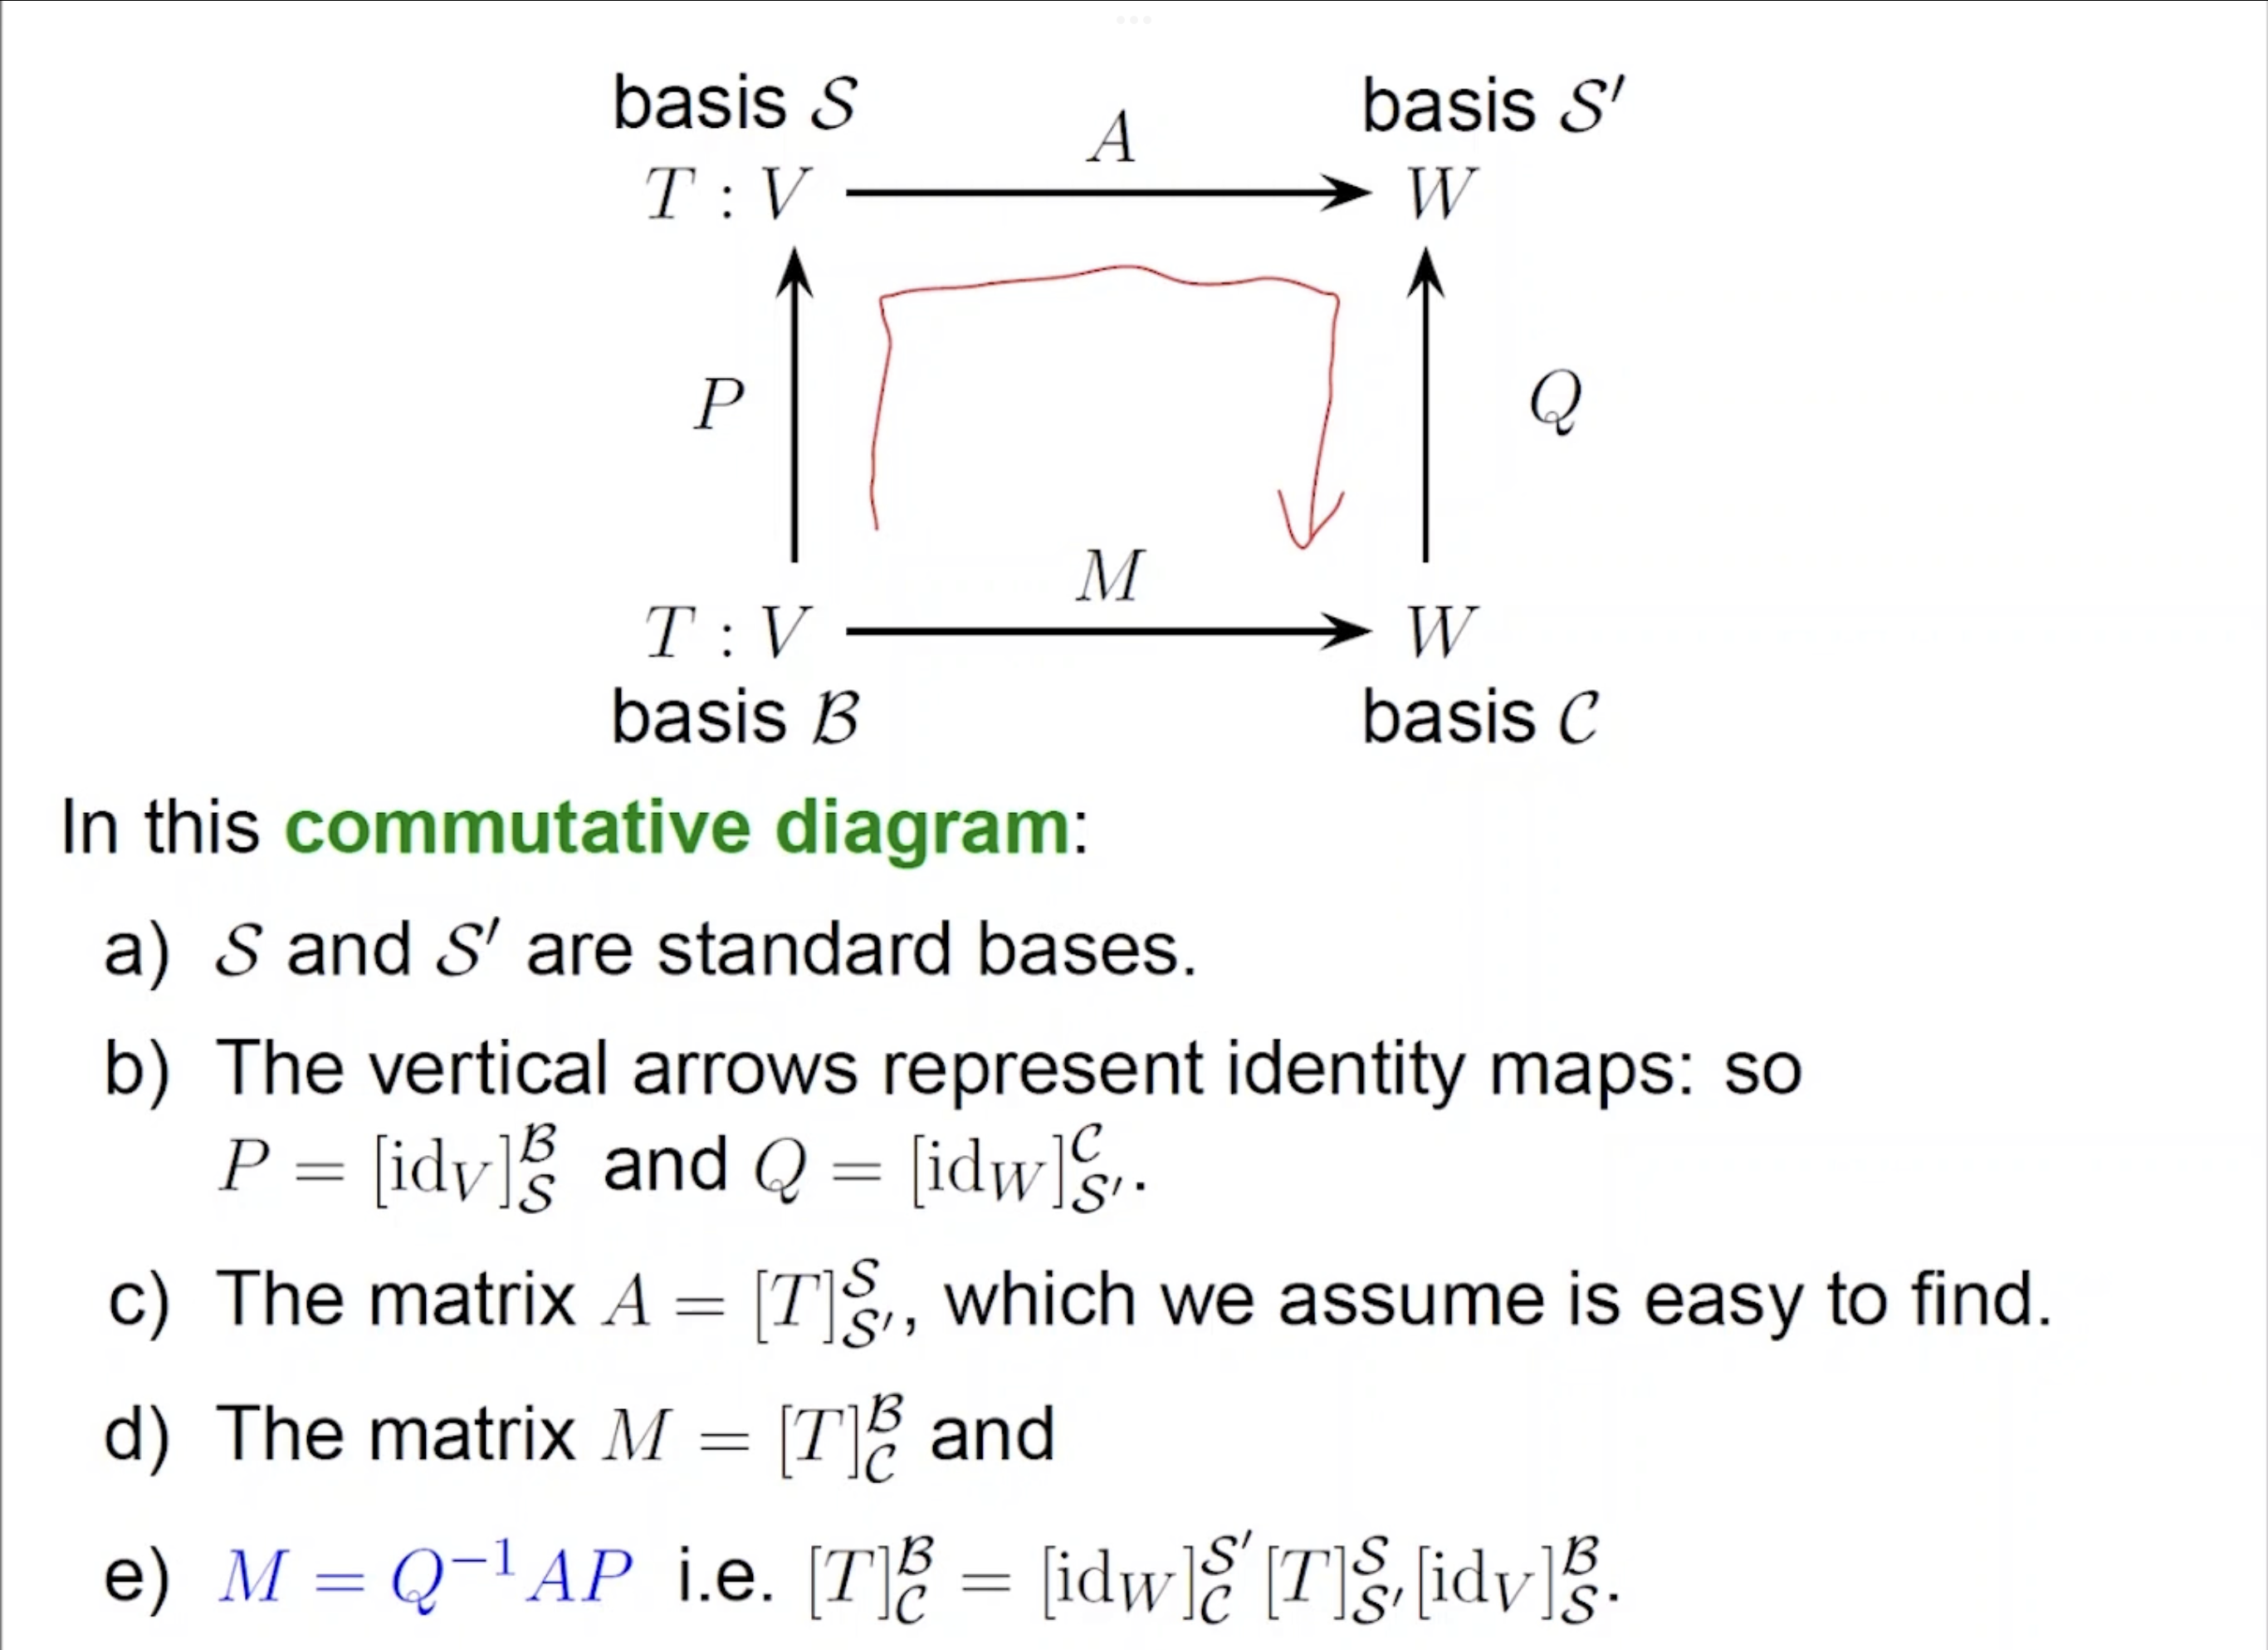
\includegraphics[scale=0.3]{assets/identity_map.png}
\end{center}
The identity maps aren't doing anything, but are easy to find and useful for changing coordinates.\newpage
\lemma{3.18}{Let $T: V \rightarrow W$ be a linear map between finite dimensional vector spaces over $\mathbb{F}$ and $A$ its matrix with respect to any two bases in $V$ and $W$.\\Then \[\text{nullity}(A) = \text{nullity}(T) \quad \text{and} \quad \text{rank}(A) = \text{rank}(T).\]\textsuperscript{*}we can see this intuitively because taking coordinates is an isomorphism.}~\\
\definition{3.7. Invariant Subspace}{Let $V$ be a vector space over $\mathbb{F}$ and $T: V \rightarrow V$ a linear map.\\If $X \leq V$ such that $T(X) \leq X$, we call $X$ an invariant subspace of $T$.}~\\
\theorem{3.19}{Let $T: V \rightarrow V$ be a linear map on a finite dimensional vector space. Suppose $V = X \oplus Y$ with both $X$ and $Y$ invariant subspaces of $T$ with dimensions $p$ and $q$ respectively.\\Then there is a basis $\mathcal{B}$ for $V$ in which the matrix $[T]^\mathcal{B}_\mathcal{B}$ of $T$ is of the form \[[T]^\mathcal{B}_\mathcal{B} = \begin{pmatrix} A & \vect{0} \\ \vect{0} & B \end{pmatrix}\]with $A$ being a $p \times p$ and $B$ a $q \times q$ matrix.}~\\
\theorem{3.20}{Let $T : V \rightarrow W$ be a linear map between finite-dimensional spaces, and let $A$ be the matrix of $T$, with respect to any bases.\\Then $T$ is invertible if and only if $A$ is invertible.\\If this is the case, then the matrix of $T^{-1}$ (with respect to the same bases) is $A^{-1}$.}~\\
\theorem{3.21}{Let $T: V \rightarrow W$ be a linear map between vector spaces over $\mathbb{F}$ where $\text{dim}(V) = p, \text{dim}(W) = q$ and $\text{rank}(T) = r$.\\Then there are bases $\mathcal{B}$ of $V$ and $\mathcal{C}$ of $W$ with respect to which the matrix of $T$ takes the form \[N_{q,p;r} = \begin{pmatrix} I_r & \vect{0} \\ \vect{0} & \vect{0} \end{pmatrix} \in M_{q,p} (\mathbb{F})\]where $I_r$ is the $r \times r$ identity matrix and $\vect{0}$ are suitably sized zero matrices.}\newpage
\corollary{3.22}{Let $A \in M_{q,p}(\mathbb{F})$ be rank $r$. Then there is a $q \times q$ invertible matrix $Q$ and a $p \times p$ invertible matrix $P$ such that \[Q^{-1}AP = N_{q,p;r}.\]}~\\
\definition{3.8. Normal Form}{The $q \times q$ rank $r$ matrix $N_{q,p;r}$ in these results is called the normal form of the map or matrix.}~\\
\definition{3.9. Similarity}{Matrices $A$ and $B$ in $M_{p,p}(\mathbb{F})$ are similar if there exists a matrix $P \in \text{GL}(p, \mathbb{F})$ such that $B = P^{-1}AP$, that is, the two matrices can be translated from each other in different bases.}~\\
\theorem{3.23}{Matrices $A_1$ and $A_2$ are similar if and only if they are the matrices of the same linear transformation with respect to two choices of bases.\\[1\baselineskip]Note that the only similar matrix to the identity map, is the identity map.}~\\
\definition{3.10. Similarity Invariant}{A property of matrices is called a similarity invariant if it is the same for all similar matrices, e.g. the determinant which is the change of the area under the mapping.}~\\
\theorem{3.24}{The rank, nullity and trace (the sum of a square matrix' diagonal elements) are all similarity invariants. (Note: so are eigenvalues, but kernels and images are, in general, not).}~\\
\definition{3.11. Multilinear Maps}{Let $V_1, V_2$ and $W$ be vector spaces over field $\mathbb{F}$. A map $T: V_1 \times V_2 \rightarrow W$ is bilinear if it is linear in each argument, that is \begin{align} T(\lambda \vect{v}_1 + {\vect{1}_1}', \vect{v}_2) &= \lambda T(\vect{v}_1, \vect{v}_2) + T( {\vect{v}_1}' + \vect{v}_2) \\ T(\vect{v}_1, \lambda \vect{v}_2 + { \vect{v}_2 }') &= \lambda T (\vect{v}_1 , \vect{v}_2 ) + T ( \vect{v}_1, { \vect{v}_2 }') \end{align} for all suitable vectors and scalars.\\If $V_2 = V_1$ we call $T$ bilinear on $V_1$.\\[\baselineskip]\textsuperscript{*}i.e. for (1), if we ignore $\vect{v}_2$ it fulfils the linearity condition, and for (2) if we ignore $\vect{v}_1$ it still fulfills the linearity condition; it is separately linear for each argument.\\[\baselineskip]\textsuperscript{**}e.g. the standard dot product, the scalar triple product on $\mathbb{R}^3$ (trilinear), the determinant.}~\\
\definition{3.12. Symmetric Multilinear Maps}{A multilinear map $T$ on $V$ is said to be symmetric if its value on any ordered set of vectors is unchanged when any two of the vectors are swapped.\\If such a swap alaways simply changes the sign of the value, $T$ is called alternating.\\[1\baselineskip]\textsuperscript{*}e.g. the dot product is symmetric since $\vect{a} \cdot \vect{b} = \vect{b} \cdot \vect{a}$; the triple scalar product is alternating.}\newpage
\definition{4.1. Positive Definite}{A bilinear $\mathbb{F}$-valued map, $T$, on $\mathbb{F}^P$ is positive definite if for all $\vect{a} \in \mathbb{F}^p, T(\vect{a}, \vect{a}) \geq 0$ and $T(\vect{a}, \vect{a}) = 0$ if and only if $a = 0$.}~\\
\theorem{4.1. Cauchy-Schwarz Inequality in $\mathbb{R}^p$}{For any $\vect{a}, \vect{b} \in \mathbb{R}^p$ we have \[- ||\vect{a}|| \; || \vect{b} || \leq \vect{a} \cdot \vect{b} \leq || \vect{a}|| \; ||\vect{b}.\]}
\corollary{4.2}{If $\vect{a} \neq \vect{0}$, $\vect{b} \neq \vect{0}$ then \[-1 \leq \frac{\vect{a} \cdot \vect{b}}{||\vect{a}|| \; || \vect{b}||} \leq 1.\]Note: In $\mathbb{R}^2, \vect{a} \cdot \vect{b} = || \vect{a} || \; || \vect{b} || \cos{\theta}$, for $0 \leq \theta \leq \pi$ the angle between the vectors.}~\\
\definition{4.2. Angle Between Vectors}{If $\vect{a}, \vect{b} \in \mathbb{R}^n$ are non-zero then the angle $\theta$ between $\vect{a}$ and $\vect{b}$ is defined by \[ \cos \theta = \frac{\vect{a} \cdot \vect{b}}{||\vect{a}|| \; || \vect{b}||}, \qquad \theta \in [0, \pi].\]We call non-zero vectors $\vect{a}$ and $\vect{b}$ orthogonal if $\vect{a} \cdot \vect{b} = 0$.}~\\
\definition{4.3. Orthogonal Component}{Let $X \leq \mathbb{R}^p$ for some $p$. The space \[Y = \{ \vect{y} \in \mathbb{R}^p : \vect{y} \cdot \vect{x} = 0 \quad \text{for all} \quad \vect{x} \in X \}\]is called the orthoginal complement of $X$, $X^{\perp}$.\\[1\baselineskip]\textsuperscript{*}i.e. it denotes another subspace orthogonal to everything in $X$.}~\\
\corollary{4.3}{For any $X \leq \mathbb{R}^p, \mathbb{R}^p = X \oplus X^\perp$ and $(X^\perp)^\perp = X$.}\newpage
\definition{4.4. Orthonormal}{A set $S = \{ \vect{v}_1, \ldots, \vect{v}_k \} \subseteq \mathbb{R}^p$ of non-zero vectors is orthogonal if $\vect{v}_i \cdot \vect{v}_j = 0, i \neq j$.\\We say $S$ is orthonormal if $\vect{v}_i \cdot \vect{v}_j = \delta{ij} = \begin{cases}
  0 & i \neq j\\
  1 & \text{otherwise}
\end{cases}$.}~\\
\lemma{4.4}{An orthogonal set $S$ in $\mathbb{R}^p$ is linearly independent.}~\\
\theorem{4.5. The Triangle Inequality}{For $\vect{a}, \vect{b} \in \mathbb{R}^p$ \[|| \vect{a} + \vect{b} || \leq ||\vect{a}|| + || \vect{b} ||.\]\textbf{Proof}: Start with $|| \vect{a} + \vect{b}||^2$ and use Cauchy-Schwarz.}~\\
\definition{4.5. Standard Dot Product in $\mathbb{C}^p$}{The standard dot product in $\mathbb{C}^p$ is defined by \[\vect{a} \cdot \vect{b} = \sum_{i=1}^p \bar{a_i}b_i = \bar{\vect{a}}^T \vect{b}.\]}~\\
\lemma{4.6}{The standard dot product in $\mathbb{C}^p$ has the following properties:
\begin{enumerate}
  \item $\vect{a} \cdot (\lambda \vect{b} + \vect{c}) = \lambda \vect{a} \cdot \vect{b} + \vect{a} \cdot \vect{c}$ for $\lambda \in \mathbb{C}$.
  \item $\vect{b} \cdot \vect{a} = \overline{\vect{a} \cdot \vect{b}}$.
  \item $(\lambda \vect{b} + \vect{c}) \cdot \vect{a} = \bar{\lambda} \vect{b} \cdot \vect{a} + \vect{c} \cdot \vect{a}$ for $\lambda \in \mathbb{C}$.
  \item $|| \vect{a} || \geq 0$ and $|| \vect{a} || = 0 \iff \vect{a} = 0$. 
\end{enumerate}}~\\
\definition{4.6. Inner Product Space}{If $V$ is a vector space over $\mathbb{F}$ then an inner product on $V$ is a function $\langle,\rangle: V \times V \rightarrow \mathbb{F}$, that is, for all $\vect{u}, \vect{v} \in V,  \langle\vect{u}, \vect{v}\rangle \in \mathbb{F}$, such that
\begin{enumerate}
  \item $\langle\vect{u}, \vect{v} + \vect{w}\rangle = \langle\vect{u}, \vect{v}\rangle + \langle\vect{u}, \vect{w}\rangle$.
  \item $\langle\vect{u}, \alpha \vect{v}\rangle = \alpha \langle\vect{u}, \vect{v}\rangle$.
  \item $\langle\vect{v}, \vect{u}\rangle = \overline{\langle\vect{u}, \vect{v}\rangle}$.
  \item $\langle\vect{v}, \vect{v}\rangle$ is real and $> 0$ if $\vect{v} \neq \vect{0}$ and $= 0$ if $\vect{v} = \vect{0}$.
\end{enumerate}
We call $V$ with $\langle , \rangle$ an inner product space. The norm of a vector is then $|| \vect{v} || = \langle \vect{v}, \vect{v} \rangle^{1/2}$.}\newpage
\lemma{4.7}{Let $V$ be an inner product space. Then for $\vect{u}, \vect{v}, \vect{w} \in V$ and $\alpha \in \mathbb{C}$:
\begin{itemize}
  \item $|| \vect{u} || > 0$ if and only if $\vect{u} \neq \vect{0}$.
  \item $\langle \vect{u} + \vect{v}, \vect{w} \rangle = \langle \vect{u}, \vect{w} \rangle + \langle \vect{v}, \vect{w} \rangle$.
  \item $\langle \alpha \vect{u}, \vect{v} \rangle = \bar{\alpha} \langle \vect{u}, \vect{v} \rangle$ and $|| \alpha \vect{u} || = | \alpha | \; || \vect{u} || $.
  \item $\langle \vect{x}, \vect{u} \rangle = 0$ for all $\vect{u}$ if and only if $\vect{x} = \vect{0}$.
  \item $| \langle \vect{u}, \vect{v} \rangle | \leq || \vect{u} || \; || \vect{v} ||$ (Cauchy-Schwarz inequality).
  \item $|| \vect{u} + \vect{v} || \leq || \vect{u} || + || \vect{v} ||$ (the triangle inequality).
\end{itemize}}~\\
\definition{4.4. Orthogonality and Orthonormality}{Let $V$ be an inner product space. Non-zero vectors $\vect{u}$ and $\vect{v}$ are orthogonal if $\langle \vect{u}, \vect{v} \rangle = 0$; we will use the notation $\vect{u} \perp \vect{v}$ for this.\\A set $S = \{ \vect{v}_1, \ldots , \vect{v}_k \} \subseteq V$ of non-zero vectors is orthogonal if $\langle \vect{v}_i, \vect{v}_j \rangle = 0, i \neq j$.\\We say $S$ is orthonormal if $\langle \vect{v}_i, \vect{v}_j \rangle = \delta_{ij} = \begin{cases} 1 & i=j \\ 0 & i \neq j \end{cases}$.\\[1\baselineskip]\textsuperscript{*}we can see that an inner product space is a generalisation for the dot product.}~\\
\definition{4.8. Projection}{In an inner product space $V$ let $\vect{v} \neq \vect{0}$.\\The projection of $\vect{u} \in V$ onto $\vect{v}$ is defined as \[ \text{proj}_\vect{v}(\vect{u}) = \frac{\langle \vect{u}, \vect{u} \rangle}{\langle \vect{v}, \vect{v} \rangle} \vect{v}.\]Note: $\vect{u} - \alpha \vect{v} \perp \vect{v} \iff \vect{u} - \alpha \vect{v} = \vect{u} - \text{proj}_\vect{v} \vect{u}$.}~\\
\lemma{4.8}{If $S = \{ \vect{v}_1, \ldots, \vect{v}_k \}$ is an orthogonal set of non-zero vectors in inner product space $V$ and $\vect{v} \in \text{span}(S)$ then $\vect{v} = \sum_{i=1}^k \text{proj}_{\vect{v}_i} \vect{v}$.\\If $S$ is an orthonormal set $\vect{v} = \sum_{i=1}^k \langle \vect{v}_i, \vect{v} \rangle \vect{v}_i$.}~\\
\corollary{4.9}{If $\{ \vect{e}_1, \ldots , \vect{e}_n \}$ is an orthonormal basis for $V$ then $\vect{v} = \sum_{i=1}^n \langle \vect{e}_i, \vect{v} \rangle \vect{e}_i$.}\newpage
\theorem{4.10. Gram-Schmidt Process}{Every finite dimensional inner product space has an orthonormal basis.\\\textbf{Proof}: Constructive. We show how to turn any given basis into an orthogonal one and then normalise.\\[1\baselineskip]
Suppose $S = \{ \vect{v}_1, \ldots, \vect{v}_p \}$ is a basis for $V$ over $\mathbb{F}$. Then let
\begin{align*}
  \vect{w}_1 &= \vect{v}_1 \notag \\
  \vect{w}_2 &= \vect{v}_2 - \text{proj}_{\vect{w}_1}(\vect{v}_2) \notag \\
  \vect{w}_3 &= \vect{v}_3 - \text{proj}_{\vect{w}_1}(\vect{v}_3) - \text{proj}_{\vect{w}_2}(\vect{v}_3) \notag \\
  \ldots \notag \\
  \vect{w}_{k+1} &= \vect{v}_{k+1} - \sum_{j=1}^k \text{proj}_{\vect{w}_j} (\vect{v}_{k+1}). \notag
\end{align*}
These resulting $\vect{w}$ vectors must be orthogonal because you subtract anything that isn't orthogonal (any overlaps). Then use an inductive hypothesis to show it is spanning.}
\end{document}